% \iffalse meta-comment
%
% Copyright (C) 2015-2020 by Josef Friedrich <josef@friedrich.rocks>
% ----------------------------------------------------------------------
% This work may be distributed and/or modified under the conditions of
% the LaTeX Project Public License, either version 1.3 of this license
% or (at your option) any later version.  The latest version of this
% license is in:
%
%   http://www.latex-project.org/lppl.txt
%
% and version 1.3 or later is part of all distributions of LaTeX
% version 2005/12/01 or later.
%
% This work has the LPPL maintenance status `maintained'.
%
% The Current Maintainer of this work is Josef Friedrich.
%
% This work consists of the files cloze.dtx and cloze.ins
% and the derived filebase cloze.sty and cloze.lua.
%
% \fi
%
% \iffalse
%<*driver>
\ProvidesFile{cloze.dtx}
%</driver>
%<package>\NeedsTeXFormat{LaTeX2e}[1999/12/01]
%<package>\ProvidesPackage{cloze}
%<*package>
    [2020/05/20 v1.4 Package to typeset cloze worksheets or cloze tests]
%</package>
%<*driver>
\documentclass{ltxdoc}
\usepackage[show]{cloze}
\usepackage{graphicx}
\usepackage{paralist}
\usepackage{titlesec}
\usepackage{mdframed}
\titleformat{\paragraph}[hang]{%
  \normalfont\normalsize\bfseries%
  }{\theparagraph}{1em}{}
\titleformat{\subparagraph}[hang]{%
  \normalfont\small\bfseries%
  }{\thesubparagraph}{1em}{}
  \titlespacing*{\subparagraph}{0pt}{*1}{0pt}

\usepackage[
  colorlinks=true,
  linkcolor=red,
  filecolor=red,
  urlcolor=red,
]{hyperref}

\MakeShortVerb{\|}

\setlength{\fboxrule}{0.2pt}
\setlength{\fboxsep}{4pt}

\makeatletter
\newcommand{\@minipagerestore}{\setlength{\parindent}{10pt}}
\makeatother

\newmdenv{example}
\definecolor{graybackground}{gray}{0.97}
\surroundwithmdframed[backgroundcolor=graybackground]{verbatim}

\newcommand{\getdefaults}[1]{%
  \directlua{tex.print(cloze.get_defaults('#1'))}%
}

\newcommand{\expdesc}[1]{(|#1|)}

\newcommand{\desc}[1]{%
  \hfill%
  \expdesc{#1}%
  \par%
}

\def\tt#1{\texttt{#1}}

\def\secref#1{(\rightarrow\ \ref{#1})}

\newcommand{\option}[2]{\tt{[#1=}\meta{#2}\tt{]}}
\newcommand{\clozeluafunction}[1]{
  \marginpar{%
    \raggedleft%
    \MacroFont%
    \tt{%
      \scantokens{\catcode`\_=12\relax#1}%
    }%
  }%
}

\newcommand{\nodelisthfont}{\bfseries\sffamily}

\newcommand{\nodelistheader}{
  \hline
  \nodelisthfont Variable name &
  \nodelisthfont Node type &
  \nodelisthfont Node subtype &
  \nodelisthfont Parameter \\
  \hline
}

\newenvironment{nodelist}{
  \noindent
  \begingroup
  \footnotesize
  \begin{tabular}{llll}
  \nodelistheader
}{
  \hline
  \end{tabular}
  \endgroup
}

\EnableCrossrefs
\CodelineIndex
\RecordChanges
\begin{document}

\providecommand*{\url}{\texttt}
\GetFileInfo{cloze.dtx}
\title{The \cloze{cloze} package%
  \thanks{Many thanks to Robert-Michael Huber for his advice
and to Paul Isambert for his article \emph{"Three things you can do with
Lua\TeX{} that would be extremely painful otherwise"} in TUGboat, Volume
31 (2010), No. 3. This article helped a lot to write this package.}%
}
\author{%
  Josef Friedrich\\%
  \url{josef@friedrich.rocks}\\%
  \href{https://github.com/Josef-Friedrich/cloze}{github.com/Josef-Friedrich/cloze}%
}
\date{\fileversion~from \filedate}

\maketitle\vfill

\pagebreak

\setcounter{secnumdepth}{5}
\setcounter{tocdepth}{5}
\tableofcontents

%-----------------------------------------------------------------------
% Introduction
%-----------------------------------------------------------------------

\pagebreak
\section{Introduction}

\emph{cloze} is a \LaTeX{} package to generate cloze texts. It uses
the capabilities of the modern \TeX{} engine \emph{Lua\TeX}. Therefore,
you must use Lua\LaTeX{} to create documents containing gaps.

\begin{verbatim}
lualatex cloze-text.tex
\end{verbatim}

The main feature of the package is that the formatting doesn't change
when using the |hide| and |show| \secref{sec:option-hide} options.

\newcommand{\clozelorem}{%
Lorem ipsum \cloze{dolor sit} amet, consectetur \cloze{adipisicing}
elit, sed do eiusmod tempor incididunt ut labore et \cloze{dolore magna}
aliqua. Ut enim ad minim veniam, quis nostrud \cloze{exercitation}
ullamco laboris nisi ut \cloze{aliquip} ex ea commodo consequat.%
}

\begin{example}
\clozelorem
\end{example}

\clozeset{hide}

The command |\clozeset{hide}| only shows gaps. When you put both texts
on top of each other you will see that they perfectly match.

\begin{example}
\clozelorem
\end{example}

\clozeset{show}

%-----------------------------------------------------------------------
% Usage
%-----------------------------------------------------------------------

\section{Usage}

There are the commands
\cmd{\cloze},
\cmd{\clozefix},
\cmd{\clozefil},
\cmd{\clozenol},
\cmd{\clozestrike} and the environments
|clozepar| and
|clozebox|
to generate cloze texts.

%%
% \cloze
%%

\subsection{The commands and environments}

\subsubsection{\cmd{\cloze}}
\label{sec:command-cloze}

\DescribeMacro{\cloze} \cmd{\cloze}\oarg{options}\marg{some text}: The
command \cmd{\cloze} is similar to a command that offers the possibility
to underline the texts. \cmd{\cloze} does not prevent line breaks. The
width of a gap depends on the number of letters and the font used.
The only option which affects the widths of a gap is the option
|margin| \secref{sec:option-margin}.

\begin{example}
Lorem ipsum \cloze{dolor} sit amet, \cloze{consectetur} adipisicing
elit, sed do eiusmod tempor incididunt ut labore et dolore
\cloze{magna aliqua. Ut enim ad minim veniam, quis nostrud exercitation
ullamco laboris nisi} ut aliquip ex ea commodo consequat.
\end{example}

\noindent It is possible to convert a complete paragraph into a `gap'.
But don't forget: There is a special environment for this: \tt{clozepar}
\secref{sec:command-clozepar}.

\begin{example}
\cloze{Lorem ipsum dolor sit amet, consectetur adipisicing elit, sed do
eiusmod tempor incididunt ut labore et dolore magna aliqua. Ut enim ad
minim veniam, quis nostrud exercitation ullamco laboris nisi ut aliquip
ex ea commodo consequat.}
\end{example}

\noindent The command \cmd{\cloze} doesn't change the behavior of the
hyphenation. Let's try some long German words:

\begin{example}
es
\cloze{Te\-le\-kom\-mu\-ni\-ka\-tions\-ü\-ber\-wach\-ung}
geht
\cloze{Un\-ter\-neh\-mens\-steu\-er\-fort\-ent\-wick\-lungs\-ge\-setz}
\cloze{Ab\-teil\-ungs\-lei\-ter\-in}
\cloze{Ober\-kom\-mi\-sar\-in}
auch
\cloze{Fil\-lial\-lei\-ter\-in}
kurz
\cloze{Ober\-kom\-mi\-sar\-in}
\cloze{Un\-ter\-neh\-mens\-steu\-er\-fort\-ent\-wick\-lungs\-ge\-setz}
\cloze{Fil\-lial\-lei\-ter\-in}
\cloze{Metz\-ger\-mei\-ster\-in}
in
\cloze{Ab\-teil\-ungs\-lei\-ter\-in}
der
\cloze{Ober\-kom\-mi\-sar\-in}
\cloze{Hoch\-lei\-stungs\-flüs\-sig\-keits\-chro\-ma\-to\-gra\-phie}
\cloze{Fil\-lial\-lei\-ter\-in}
Kürze
\cloze{Un\-ter\-neh\-mens\-steu\-er\-fort\-ent\-wick\-lungs\-ge\-setz}
\cloze{Metz\-ger\-mei\-ster\-in}
liegt
\cloze{Ab\-teil\-ungs\-lei\-ter\-in}
die
\cloze{Metz\-ger\-mei\-ster\-in}
\cloze{Ab\-teil\-ungs\-lei\-ter\-in}
Würze
\cloze{Ober\-kom\-mi\-sar\-in}
\end{example}

%%
% \clozesetfont
%%

\subsubsection{\cmd{\clozesetfont}}
\label{sec:command-clozesetfont}
\label{sec:command-clozefont}

\DescribeMacro{\clozesetfont}
The gap font can be changed by using the command
\cmd{\clozesetfont}. \tt{\string\cloze\-set\-font} redefines the command
\cmd{\clozefont} which contains the font definition.
Thus, the command \tt{\string\clozesetfont\string{\string\Large\string}}
has the same effect as
\tt{\string\re\-new\-com\-mand\string{\string\cloze\-font\string}%
\string{\string\Large\string}}.

\clozesetfont{\Large}

\begin{example}
Excepteur \cloze{sint} occaecat \cloze{cupidatat} non proident.
\end{example}

\noindent Please do not put any color definitions in
\cmd{\clozesetfont}, as it won't work. Use the option
|textcolor| instead \secref{sec:option-textcolor}.

|\clozesetfont{\ttfamily\normalsize}| changes the gap text for example
into a normal sized typewriter font.

\clozesetfont{\ttfamily\normalsize}

\begin{example}
Excepteur \cloze{sint} occaecat \cloze{cupidatat} non proident.
\end{example}

\clozesetfont{\itshape}

%%
% \clozefix
%%

\subsubsection{\cmd{\clozefix}}
\label{sec:command-clozefix}

\DescribeMacro{\clozefix} \cmd{\clozefix}\oarg{options}\marg{some text}:
The command \cmd{\clozefix} creates gaps with a fixed width. The
clozes are default concering the width \tt{\getdefaults{width}}.

\begin{example}
\noindent Lorem ipsum dolor sit amet:
\begin{compactenum}
\item \clozefix[width=5cm]{consectetur}
\item \clozefix[width=5cm]{adipisicing}
\item \clozefix[width=5cm]{elit}
\end{compactenum}
sed do eiusmod.
\end{example}

Gaps with a fixed width are much harder to solve.

\begin{example}
Lorem ipsum dolor \clozefix[align=center,width=3cm]{sit} amet,
\clozefix[align=center,width=3cm]{consectetur} adipisicing elit, sed do
eiusmod tempor incididunt \clozefix[align=center,width=3cm]{ut} labore
et dolore magna aliqua.
\end{example}

Using the option |align| you can make nice tabulars like this:

\begin{example}
\begin{tabular}{p{5cm}p{4cm}}
\raggedleft Composer & Life span \\
\clozefix[width=5cm,align=right]{Joseph Haydn} & \clozefix{1723-1809} \\
\clozefix[width=5cm,align=right]{Wolfgang Amadeus Mozart} & \clozefix{1756-1791} \\
\clozefix[width=5cm,align=right]{Ludwig van Beethoven} & \clozefix{1770-1827} \\
\end{tabular}
\end{example}

%%
% \clozenol
%%

\subsubsection{\cmd{\clozenol}}
\label{sec:command-clozenol}
\DescribeMacro{\clozenol} \cmd{\clozenol}\oarg{options}\marg{some text}:
The macro name |clozenol| stands for \emph{“cloze no line”}. As the
the name suggests this macro typesets cloze texts without a line.

\begin{verbatim}
Lorem \clozenol{ipsum dolor} sit amet.
\end{verbatim}

\begin{example}
Lorem \clozenol{ipsum dolor} sit amet.
\end{example}

\begin{verbatim}
Lorem \clozenol[textcolor=green]{ipsum dolor} sit amet.
\end{verbatim}

\begin{example}
Lorem \clozenol[textcolor=green]{ipsum dolor} sit amet.
\end{example}

%%
% \clozefil
%%

\subsubsection{\cmd{\clozefil}}
\label{sec:command-clozefil}

\DescribeMacro{\clozefil} \cmd{\clozefil}\oarg{options}\marg{some text}:
The name of the command is inspired by \cmd{\hfil}, \cmd{\hfill}, and
\cmd{\hfilll}. Only \cmd{\clozefil} fills out all available horizontal
spaces with a line.

\begin{example}
Lorem ipsum dolor sit amet, \clozefil{consectetur adipisicing elit, sed
do eiusmod.}

Ut enim \clozefil{ad minim veniam} exercitation.
\end{example}

%%
% \clozeextend
%%

\subsubsection{\cmd{\clozeextend}}
\label{sec:command-clozeextend}

\DescribeMacro{\clozeextend} \cmd{\clozeextend}\oarg{spaces}:
The command |\clozeextend| adds some invisible placeholders to extend
some cloze texts with blank space.

\begin{verbatim}
\begin{itemize}
\item \clozefil{Lorem ipsum dolor sit amet, consectetur adipisicing
elit, sed do eiusmod tempor incididunt ut labore et dolore magna
aliqua.}
\item \clozefil{Ut enim ad minim veniam \clozeextend[20]}
\item \clozefil{quis nostrud \clozeextend[20]}
\end{itemize}
\end{verbatim}

\begin{example}
\begin{itemize}
\item \clozefil{Lorem ipsum dolor sit amet, consectetur adipisicing
elit, sed do eiusmod tempor incididunt ut labore et dolore magna
aliqua.}
\item \clozefil{Ut enim ad minim veniam \clozeextend[20]}
\item \clozefil{quis nostrud \clozeextend[20]}
\end{itemize}
\end{example}

%%
% clozepar
%%

\subsubsection{\tt{clozepar}}
\label{sec:command-clozepar}

\DescribeEnv{clozepar} |\begin{clozepar}|\oarg{options} \dots
\textit{some text} \dots |\end{clozepar}|: The environment \tt{clozepar}
transforms a complete paragraph into a cloze text. The options |align|,
|margin| and |width| have no effect on this environment.

\begin{example}
Lorem ipsum dolor sit amet, consectetur adipisicing elit ullamco laboris
nisi.

\begin{clozepar}
Ut enim ad minim veniam, quis nostrud exercitation ullamco laboris nisi
ut aliquip ex ea commodo consequat. Duis aute irure dolor in
reprehenderit in voluptate velit esse cillum.
\end{clozepar}

Excepteur sint occaecat cupidatat non proident.
\end{example}

%%
% clozebox
%%

\subsubsection{\tt{clozebox}}
\label{sec:command-clozebox}

\DescribeEnv{clozebox} |\begin{clozebox}|*\oarg{options} \dots
\textit{some text} \dots |\end{clozebox}|: The environment \tt{clozebox}
surrounds a text with a box. The starred version omits the line
around the box. Use the options |boxwidth| and |boxheight| to specify
the dimensions of the box. By default the width of the box is
|\linewidth|.

\begin{verbatim}
\begin{clozebox}
Lorem ipsum dolor sit amet, consectetur adipisicing elit, sed do eiusmod
tempor incididunt ut labore et dolore magna aliqua.
\end{clozebox}
\end{verbatim}

\bigskip
\noindent
|\clozehide|
\clozehide
\bigskip

\begin{center}
\begin{clozebox}[boxwidth=8cm]
Lorem ipsum dolor sit amet, consectetur adipisicing elit, sed do eiusmod
tempor incididunt ut labore et dolore magna aliqua.
\end{clozebox}
\end{center}

\bigskip
\noindent
|\clozeshow|
\clozeshow
\bigskip

\begin{center}
\begin{clozebox}[boxwidth=8cm]
Lorem ipsum dolor sit amet, consectetur adipisicing elit, sed do eiusmod
tempor incididunt ut labore et dolore magna aliqua.
\end{clozebox}
\end{center}

\paragraph{Option boxwidth}
\label{sec:command-clozebox-boxwidth}
See the documentation about the option \secref{sec:option-boxwidth}.

\begin{verbatim}
\begin{clozebox}[boxwidth=5cm]
Lorem ipsum dolor sit amet, consectetur adipisicing elit, sed do eiusmod
tempor incididunt ut labore et dolore magna aliqua.
\end{clozebox}
\end{verbatim}

\begin{center}
\begin{clozebox}[boxwidth=5cm]
Lorem ipsum dolor sit amet, consectetur adipisicing elit, sed do eiusmod
tempor incididunt ut labore et dolore magna aliqua.
\end{clozebox}
\end{center}

\paragraph{Option boxheight}
\label{sec:command-clozebox-boxheight}
See the documentation about the option \secref{sec:option-boxheight}.

\begin{verbatim}
\begin{clozebox}[boxwidth=5cm,boxheight=5cm]
Lorem ipsum dolor sit amet, consectetur adipisicing elit, sed do eiusmod
tempor incididunt ut labore et dolore magna aliqua.
\end{clozebox}
\end{verbatim}

\begin{center}
\begin{clozebox}[boxwidth=5cm,boxheight=5cm]
Lorem ipsum dolor sit amet, consectetur adipisicing elit, sed do eiusmod
tempor incididunt ut labore et dolore magna aliqua.
\end{clozebox}
\end{center}

\paragraph{starred}

% starred
\begin{verbatim}
\begin{clozebox}*[boxwidth=5cm,boxheight=5cm]
Lorem ipsum dolor sit amet, consectetur adipisicing elit, sed do eiusmod
tempor incididunt ut labore et dolore magna aliqua.
\end{clozebox}
\end{verbatim}

\begin{center}
\begin{clozebox}*[boxwidth=5cm,boxheight=5cm]
Lorem ipsum dolor sit amet, consectetur adipisicing elit, sed do eiusmod
tempor incididunt ut labore et dolore magna aliqua.
\end{clozebox}
\end{center}

%%
% clozespace
%%

\subsubsection{\tt{clozespace}}
\label{sec:command-clozespace}

\DescribeEnv{clozespace} |\begin{clozespace}|\oarg{options} \dots
\textit{some text} \dots |\end{clozespace}|

\begin{verbatim}
\begin{clozespace}[spacing=2]
\clozesetfont{\ttfamily\Huge}
Lorem \cloze{ipsum} dolor sit \cloze{amet}, consectetur adipisicing
elit, sed do eiusmod tempor incididunt ut labore et dolore magna
aliqua. Ut enim ad minim veniam, quis \cloze{nostrud}
exercitation ullamco \cloze{laboris} nisi ut aliquip ex ea commodo
consequat.
\end{clozespace}
\end{verbatim}

\begin{example}
\begin{clozespace}[spacing=2]
\clozesetfont{\ttfamily\Huge}
Lorem \cloze{ipsum} dolor sit \cloze{amet}, consectetur adipisicing
elit, sed do eiusmod tempor incididunt ut labore et dolore magna
aliqua. Ut enim ad minim veniam, quis \cloze{nostrud}
exercitation ullamco \cloze{laboris} nisi ut aliquip ex ea commodo
consequat.
\vspace{-0.8cm}
\end{clozespace}
\end{example}

%%
% \clozeline
%%

\subsubsection{\cmd{\clozeline}}
\label{sec:command-clozeline}

\DescribeMacro{\clozeline}
\cmd{\clozeline}\oarg{options}:
To create a cloze line of a certain width, use the command
\cmd{\clozeline}. The default width of the line is
\tt{\getdefaults{width}}. In combination with the other cloze commands
you can create for example an irregular alignment of the cloze text.

\begin{verbatim}
Ut enim ad
\clozeline[width=1cm]\cloze{minim}\clozeline[width=3cm]
minim veniam
\end{verbatim}

\begin{example}
Ut enim ad \clozeline[width=1cm]\cloze{minim}\clozeline[width=3cm] minim
veniam,
\end{example}

%%
% \clozelinefil
%%

\subsubsection{\cmd{\clozelinefil}}
\label{sec:command-clozelinefil}

\DescribeMacro{\clozelinefil}
\cmd{\clozelinefil}\oarg{options}:
This command \cmd{\clozelinefil} fills the
complete available horizontal space with a line. Moreover,
\cmd{\clozelinefil} was used to create \cmd{\clozefil}.

\begin{example}
Lorem\clozelinefil
\end{example}

%%
% \clozestrike
%%

\subsubsection{\cmd{\clozestrike}}
\label{sec:command-clozelinefil}

\DescribeMacro{\clozestrike}
\cmd{\clozestrike}\oarg{options}\marg{wrong text}\marg{correct text}

\begin{verbatim}
Lorem \clozestrike{ipsum}{dolor} sit amet.
\end{verbatim}

\begin{example}
Lorem \clozestrike{ipsum}{dolor} sit amet.
\end{example}

\begin{verbatim}
Lorem \clozestrike[textcolor=red]{ipsum}{dolor} sit amet.
\end{verbatim}

\begin{example}
Lorem \clozestrike[textcolor=red]{ipsum}{dolor} sit amet.
\end{example}

\begin{example}
\begin{clozespace}
invidunt ut \clozestrike{labore}{et dolore magna aliquyam erat}, sed
diam voluptua. At \clozestrike{vero eos}{et accusam et justo} duo
dolores et ea \clozestrike{rebum. Stet}{clita kasd gubergren}, no sea
takimata sanctus est Lorem ipsum dolor sit amet. Lorem ipsum
\clozestrike{dolor sit amet, consetetur }{sadipscing elitr, sed diam}
nonumy eirmod tempor invidunt ut labore et dolore magna
aliquyam erat, \clozestrike{sed diam voluptua}{At vero}.
\end{clozespace}
\end{example}

\begin{example}
\clozehide
\begin{clozespace}
invidunt ut \clozestrike{labore}{et dolore magna aliquyam erat}, sed
diam voluptua. At \clozestrike{vero eos}{et accusam et justo} duo
dolores et ea \clozestrike{rebum. Stet}{clita kasd gubergren}, no sea
takimata sanctus est Lorem ipsum dolor sit amet. Lorem ipsum
\clozestrike{dolor sit amet, consetetur }{sadipscing elitr, sed diam}
nonumy eirmod tempor invidunt ut labore et dolore magna
aliquyam erat, \clozestrike{sed diam voluptua}{At vero}.
\end{clozespace}
\clozeshow
\end{example}

%-----------------------------------------------------------------------
% Options
%-----------------------------------------------------------------------

\subsection{The options}

%%
% Local and global options
%%

\subsubsection{Local and global options}

The \emph{cloze} package distinguishs between \emph{local} and
\emph{global} options. Besides the possiblity to set \emph{global}
options in the \cmd{\usepackage}\oarg{global options}\marg{cloze}
declaration, the cloze package offers a special command to set
\emph{global} options:
\cmd{\clozeset}\marg{global options}

%%
% \clozeset
%%

\subsubsection{\cmd{\clozeset}}
\label{sec:command-clozeset}

\DescribeMacro{\clozeset}
\cmd{\clozeset}\marg{global options}: The command can set \emph{global}
options for each paragraph.

\begin{verbatim}
\clozeset{textcolor=red} Lorem \cloze{ipsum} dolor \par
\clozeset{textcolor=green} Lorem \cloze{ipsum} dolor
\end{verbatim}

\begin{example}
\clozeset{textcolor=red} Lorem \cloze{ipsum} dolor \par
\clozeset{textcolor=green} Lorem \cloze{ipsum} dolor
\end{example}

\noindent \cmd{\clozeset} does not change the options within a
paragraph. As you can see in the example below the last \cmd{\clozeset}
applies the color green for both gaps.

\begin{verbatim}
\clozeset{textcolor=red} Lorem \cloze{ipsum} dolor
\clozeset{textcolor=green} Lorem \cloze{ipsum} dolor
\end{verbatim}

\begin{example}
\clozeset{textcolor=red} Lorem \cloze{ipsum} dolor
\clozeset{textcolor=green} Lorem \cloze{ipsum} dolor
\end{example}

\clozereset

%%
% \clozereset
%%

\subsubsection{\cmd{\clozereset}}
\label{sec:command-clozereset}

\DescribeMacro{\clozereset}
\cmd{\clozereset}: The command resets all \emph{global} options to the
default values. It has no effect on the \emph{local} options.

\begin{verbatim}
\clozeset{
  thickness=3mm,
  linecolor=yellow,
  textcolor=magenta,
  margin=-2pt
}
\end{verbatim}

\clozeset{thickness=3mm,linecolor=yellow,textcolor=magenta,margin=-2pt}

\begin{example}
Very \cloze{silly} global \cloze{options}.
\end{example}

\begin{verbatim}
\clozereset
\end{verbatim}
\clozereset

\begin{example}
\cloze{Relax!} We can reset \cloze{those} options.
\end{example}

%%
% \clozereset
%%

\subsubsection{\cmd{\clozeshow} and \cmd{\clozehide}}
\label{sec:command-clozeshow}
\label{sec:command-clozehide}

\DescribeMacro{\clozeshow} \DescribeMacro{\clozehide}
\cmd{\clozeshow} and \cmd{\clozehide}: This commands are shortcuts for
\cmd{\clozeset}\marg{show} and \cmd{\clozeset}\marg{hide}.

\begin{verbatim}
\clozehide
\end{verbatim}
\clozehide

\begin{example}
Lorem \cloze{ipsum dolor sit} amet, consectetur \cloze{adipisicing}
elit.
\end{example}

\begin{verbatim}
\clozeshow
\end{verbatim}
\clozeshow

\begin{example}
Lorem \cloze{ipsum dolor sit} amet, consectetur \cloze{adipisicing}
elit.
\end{example}

%%
% align
%%

\subsubsection{\tt{align}}
\label{sec:option-align}

\option{align}{left/center/right}:
Only the macro \cmd{\clozefix} \secref{sec:command-clozefix} takes the
option \tt{align} into account. Possible values are \tt{left},
\tt{center} and \tt{right}. This option only makes sense, if the width
of the line is larger than the width of the text.

\newcommand{\optionsalign}[1]{%
  \noindent%
  \clozefix[align=#1,width=8cm]{Lorem ipsum}%
  \desc{#1}%
}

\begin{example}
\optionsalign{left}
\optionsalign{center}
\optionsalign{right}
\end{example}

%%
% boxheight
%%

\subsubsection{\tt{boxheight}}
\label{sec:option-boxheight}

|boxheight| specifies the height of a cloze box. This option has only
an effect on the environment |clozebox| \secref{sec:command-clozebox}.
An example can be found in the section about the environment
\secref{sec:command-clozebox-boxheight}.

%%
% boxwidth
%%

\subsubsection{\tt{boxwidth}}
\label{sec:option-boxwidth}

|boxwidth| specifies the width of a cloze box. This option has only
an effect on the environment |clozebox| \secref{sec:command-clozebox}.
An example can be found in the section about the environment
\secref{sec:command-clozebox-boxwidth}.

%%
% distance
%%

\subsubsection{\tt{distance}}
\label{sec:option-distance}

\option{distance}{dimen}:
The option |distance| specifies the spacing between the baseline of the
text and the gap line. The larger the dimension of the option
|distance|, the more moves the line down. Negative values cause the line
to appear above the baseline. The default value is
\tt{\getdefaults{distance}}.

\newcommand{\optiondistance}[1]{%
  \noindent%
  \clozefil[distance=#1]{Lorem ipsum dolor sit amet.}
  \expdesc{#1}
  \par%
}

\begin{example}
\optiondistance{\getdefaults{distance}}
\optiondistance{3pt}
\optiondistance{-3pt}
\end{example}

%%
% hide and show
%%

\subsubsection{\tt{hide} and \tt{show}}
\label{sec:option-hide}
\label{sec:option-show}

\tt{[hide]} and \tt{[show]}:
By default the cloze text is displayed. Use the option |hide| to remove
the cloze text from the output.  If you accidentally specify both
options -- |hide| and |show| -- the last option "wins".

\newcommand{\optionshow}[1]{%
  \noindent%
  Lorem ipsum \cloze[#1]{dolor sit amet}, consectetur
  \cloze[#1]{adipisicing} elit.%
  \desc{#1}%
}

\begin{example}
\optionshow{hide}
\optionshow{show}
\optionshow{show,hide}
\optionshow{hide,show}
\end{example}

%%
% linecolor and textcolor
%%

\subsubsection{\tt{linecolor} and \tt{textcolor}}
\label{sec:option-linecolor}
\label{sec:option-textcolor}

\option{linecolor}{color name} and
\option{textcolor}{color name}:
Values for both color options are color names used by the xcolor
package. To define your own color use the following command:

\begin{verbatim}
\definecolor{myclozecolor}{rgb}{0.1,0.4,0.6}
\cloze[textcolor=myclozecolor]{Lorem ipsum}
\end{verbatim}
\definecolor{myclozecolor}{rgb}{0.1,0.4,0.6}

\newcommand{\optioncolor}[2]{%
  \noindent%
  \clozefil[#1=#2]{Lorem ipsum dolor sit amet, consectetur} %
  \expdesc{#2}%
  \par%
}

\begin{example}
\optioncolor{textcolor}{myclozecolor}
\optioncolor{textcolor}{red}
\optioncolor{textcolor}{green}
\end{example}

\noindent You can use the same color names to colorize the cloze lines.

\begin{example}
\optioncolor{linecolor}{myclozecolor}
\optioncolor{linecolor}{red}
\optioncolor{linecolor}{green}
\end{example}

%%
% margin
%%

\subsubsection{\tt{margin}}
\label{sec:option-margin}

\option{margin}{dimen}:
The option |margin| indicates how far the line sticks up from the text.
The option can be used with the commands \cmd{\cloze}, \cmd{\clozefix}
and \cmd{\clozefil}. The default value of the option is
\tt{\getdefaults{margin}}.

\newcommand{\optionmargin}[1]{%
  \noindent%
  Lorem ipsum \cloze[margin=#1]{dolor} sit amet.%
  \desc{#1}%
}

\begin{example}
\optionmargin{0pt}
\optionmargin{5mm}
\optionmargin{1cm}
\optionmargin{6em}
\optionmargin{-4pt}
\end{example}

% Folgt ein Satzzeichen direkt auf eine Lücke, so findet der
% Zeilenumbruch erst nach dem Satzzeichen statt. Auch ein noch so großer
% Wert für |margin| beeinflusst dieses Verhalten nicht.
\noindent Is a punctation mark placed directly after a gap, then the
line breaks after this punctation mark. Even the most large value of
|margin| does not affect this behavior.

\begin{example}
\clozeset{margin=3mm}
\cloze{Lorem}, \cloze{ipsum}. \cloze{dolor}; \cloze{sit}: \cloze{amet},
\cloze{consectetur}. \cloze{adipisicing}; \cloze{elit}: \cloze{sed},
\cloze{do}. \cloze{eiusmod}; \cloze{tempor}.
\end{example}

\clozereset

%%
% spacing
%%

\subsubsection{\tt{spacing}}
\label{sec:option-spacing}

\option{spacing}{number}: This option provides support for setting the
spacing  between lines. A larger font used for the cloze texts needs
more line space to avoid unsteady line distances.
This option only affects the environment |clozespace|
\secref{sec:command-clozespace}.

%%
% thickness
%%

\subsubsection{\tt{thickness}}
\label{sec:option-thickness}

\option{thickness}{dimen}:
The option |thickness| indicates how thick the line is. The option
|distance| \secref{sec:option-distance} is not affected by this option,
because the bottom of the line moves down. The default value of this
option is \tt{\getdefaults{thickness}}.

\newcommand{\optionthickness}[1]{%
  \noindent%
  Lorem \cloze[thickness=#1]{ipsum dolor sit} amet.%
  \desc{#1}%
}

\begin{example}
\optionthickness{0.01pt}
\optionthickness{1pt}
\optionthickness{2pt}
\end{example}

%%
% width
%%

\subsubsection{\tt{width}}\label{sec:option-width}

\option{width}{dimen}:
The only command which can be changed by the option |width| is
\cmd{\clozefix} \secref{sec:command-clozefix}. The default value of the
option is \tt{\getdefaults{width}}.

\newcommand{\optionwidth}[1]{%
  \noindent%
  Lorem \clozefix[width=#1]{dolor} amet.%
  \desc{#1}%
}

\begin{example}
\optionwidth{3cm}
\optionwidth{5cm}
\optionwidth{7cm}
\end{example}

%-----------------------------------------------------------------------
% Special application areas
%-----------------------------------------------------------------------

\subsection{Special application areas}

%%
% tabbing
%%

\subsubsection{The \tt{tabbing} environment}

\begin{verbatim}
\begin{tabbing}
col1 \hspace{1cm} \= col2 \hspace{1cm} \= col3 \hspace{1cm} \= col4 \\
\cloze{col1} \> \> \clozefix{col3} \\
\end{tabbing}
\end{verbatim}

\begin{example}
\begin{tabbing}
col1 \hspace{1cm} \= col2 \hspace{1cm} \= col3 \hspace{1cm} \= col4 \\
\cloze{col1} \> \> \clozefix{col3} \\
\end{tabbing}
\end{example}

%%
% picture
%%

\subsubsection{The \tt{picture} environment}

\begin{verbatim}
\begin{picture}(320,100)
\put(80,25){\cloze{Lorem}}
\put(160,50){\clozefix{ipsum}}
\put(240,75){\clozefil{dolor}}
\end{picture}
\end{verbatim}

\begin{example}
\begin{picture}(320,100)
\put(80,25){\cloze{Lorem}}
\put(160,50){\clozefix{ipsum}}
\put(240,75){\clozefil{dolor}}
\end{picture}
\end{example}

%%
% tabular
%%

\subsubsection{The \tt{tabular} environment}

\begin{verbatim}
\begin{tabular}{l c}
\cloze{Lorem} & \cloze{ipsum} \\
\clozefix{amet} & \clozefix{consectetur} \\
\cloze{sed} & \cloze{do} \\
\end{tabular}
\end{verbatim}

% No |c| inside because of short verbatim.

\begin{example}
\clozeset{width=1cm}
\begin{tabular}{l c}
\cloze{Lorem} & \cloze{ipsum} \\
\clozefix{amet} & \clozefix{consectetur} \\
\cloze{sed} & \cloze{do} \\
\end{tabular}
\end{example}

  \DocInput{cloze.dtx}
  \pagebreak
  \PrintChanges
  \pagebreak
  \PrintIndex
\end{document}
%</driver>
%<*readme>
# Description

EN: `cloze` is a LuaLaTeX/LaTeX package to generate cloze. It uses the
capabilities of the modern TeX engine LuaTex.

DE: `cloze` ist a LuaLaTeX/LaTeX-Paket zum Erstellen von Lückentexten.
Es nutzt die Möglichkeiten der modernen TeX-Engine LuaTeX.

# License

Copyright (C) 2015-2020 by Josef Friedrich <josef@friedrich.rocks>
------------------------------------------------------------------------
This work may be distributed and/or modified under the conditions of
the LaTeX Project Public License, either version 1.3 of this license
or (at your option) any later version.  The latest version of this
license is in:

  http://www.latex-project.org/lppl.txt

and version 1.3 or later is part of all distributions of LaTeX
version 2005/12/01 or later.

# CTAN

Since July 2015 the cloze package is included in the Comprehensive TeX
Archive Network (CTAN).

* TeX archive: http://mirror.ctan.org/tex-archive/macros/luatex/latex/cloze
* Package page: https://www.ctan.org/pkg/cloze

# Repository

https://github.com/Josef-Friedrich/cloze

# Installation

Get source:

    git clone git@github.com:Josef-Friedrich/cloze.git
    cd cloze

Compile:

    make

or manually:

    luatex cloze.ins
    lualatex cloze.dtx
    makeindex -s gglo.ist -o cloze.gls cloze.glo
    makeindex -s gind.ist -o cloze.ind cloze.idx
    lualatex cloze.dtx

# Development

First delete the stable version installed by TeX Live. Because the
package `cloze` belongs to the collection `collection-latexextra`, the
option  `--force` must be used to delete the package.

    tlmgr remove --force cloze

## Deploying a new version

Update the version number on this locations in the file `cloze.dtx`

### `cloze.sty` (approximately at the line number 30)

    %<*package>
      [2020/05/20 v1.4 Package to typeset cloze worksheets or cloze tests]
    %<*package>

### documentation  (approximately at the line number 1250)

Add a changes entry:

```latex
\changes{v1.4}{2020/05/20}{...}
```

### `cloze.lua` (approximately at the line number 1900)

```lua
if not modules then modules = { } end modules ['cloze'] = {
  version   = '1.4'
}
```

### Update the copyright year:

```
sed -i 's/(C) 2015-2020/(C) 2015-2021/g' cloze.ins
sed -i 's/(C) 2015-2020/(C) 2015-2021/g' cloze.dtx
```

### Command line tasks:

```
git tag v1.4
make
make ctan
```
%</readme>
% \fi
%
% \CheckSum{0}
%
% \CharacterTable
%  {Upper-case    \A\B\C\D\E\F\G\H\I\J\K\L\M\N\O\P\Q\R\S\T\U\V\W\X\Y\Z
%   Lower-case    \a\b\c\d\e\f\g\h\i\j\k\l\m\n\o\p\q\r\s\t\u\v\w\x\y\z
%   Digits        \0\1\2\3\4\5\6\7\8\9
%   Exclamation   \!     Double quote  \"     Hash (number) \#
%   Dollar        \$     Percent       \%     Ampersand     \&
%   Acute accent  \'     Left paren    \(     Right paren   \)
%   Asterisk      \*     Plus          \+     Comma         \,
%   Minus         \-     Point         \.     Solidus       \/
%   Colon         \:     Semicolon     \;     Less than     \<
%   Equals        \=     Greater than  \>     Question mark \?
%   Commercial at \@     Left bracket  \[     Backslash     \\
%   Right bracket \]     Circumflex    \^     Underscore    \_
%   Grave accent  \`     Left brace    \{     Vertical bar  \|
%   Right brace   \}     Tilde         \~}
%
%
% \changes{v0.1}{2015/06/16}{Converted to DTX file}
% \changes{v1.0}{2015/07/08}{Inital release}
% \changes{v1.1}{2016/06/13}{Make cloze compatible to LuaTeX version
% 0.95}
% \changes{v1.2}{2016/06/23}{The cloze makros are now working in
% tabular, tabbing and picture environments}
% \changes{v1.3}{2017/03/13}{Add the new macros \cmd{\clozenol} and
% \cmd{\clozeextend} and the environments \texttt{clozebox} and
% \texttt{clozespace} (This version was not published on CTAN.)}
% \changes{v1.4}{2020/05/20}{Add the new macro \cmd{\clozestrike} and
% improve the documentation}
%
% \DoNotIndex{\newcommand,\newenvironment,\def,\directlua}
%
% \StopEventually{}
% \pagebreak
% \section{Implementation}
%
% \iffalse
%<*package>
% \fi
% \MacroTopsep = 10pt plus 2pt minus 2pt
% \MacrocodeTopsep = 10pt plus 1.2pt minus 1pt
%
% \makeatletter
% \c@CodelineNo 25 \relax
% \makeatother
%
% \subsection{The file \tt{cloze.sty}}
%
% This packages are used to build \emph{cloze}:
%
% \subsubsection{Dependencies}
%
% The package \href{https://www.ctan.org/pkg/fontspec}{fontspec} is not
% necessarily required. When using Lua\LaTeX{} it is good form to load
% it. Apart from this the package supplies helpful messages, when you
% compile a Lua\LaTeX{} document with pdf\LaTeX{}.
%    \begin{macrocode}
\RequirePackage{fontspec}
%    \end{macrocode}
% The package \href{https://www.ctan.org/pkg/luatexbase}{luatexbase}
% allows to register multiple Lua callbacks.
%    \begin{macrocode}
\RequirePackage{luatexbase-mcb}
%    \end{macrocode}
% The package \href{https://www.ctan.org/pkg/kvoptions}{kvoptions}
% takes the handling of the options.
%    \begin{macrocode}
\RequirePackage{kvoptions}
%    \end{macrocode}
% The package \href{https://www.ctan.org/pkg/setspace}{setspace} is used
% by the environment |clozespace|.
%    \begin{macrocode}
\RequirePackage{setspace}
%    \end{macrocode}
% The package \href{https://www.ctan.org/pkg/xcolor}{xcolor} is required
% to colorize the text and the line of a gap.
%    \begin{macrocode}
\RequirePackage{xcolor}
%    \end{macrocode}
% The package \href{https://www.ctan.org/pkg/xcolor}{xparse} is used by
% the environment |clozebox|.
%    \begin{macrocode}
\RequirePackage{xparse}
%    \end{macrocode}
% The package \href{https://www.ctan.org/pkg/stackengine}{stackengine}
% is required by the command |\clozestrike{}{}|.
%    \begin{macrocode}
\RequirePackage{stackengine}
%    \end{macrocode}
% The package \href{https://www.ctan.org/pkg/ulem}{ulem} is required by
% the command |\clozestrike{}{}|.
%    \begin{macrocode}
\RequirePackage{ulem}
\normalem
%    \end{macrocode}
%
%    \begin{macrocode}
\RequirePackage{transparent}
%    \end{macrocode}
%
% Load the cloze lua module and put all return values in the variable
% |cloze|.
%
%    \begin{macrocode}
\directlua{
  cloze = require('cloze')
}
%    \end{macrocode}
%
%    \begin{macrocode}
\newif\ifclozeshow\clozeshowtrue
%    \end{macrocode}
%
% \subsubsection{Internal macros}
%
% \begin{macro}{\cloze@set@to@global}
% Set the Lua variable |registry.is_global| to |true|. All options
% are then stored in the variable |registry.global_options|.
%    \begin{macrocode}
\def\cloze@set@to@global{%
 \directlua{cloze.set_is_global(true)}%
}
%    \end{macrocode}
% \end{macro}
%
% \begin{macro}{\cloze@set@to@local}
% First unset the variable |registry.local_options|. Now set the Lua
% variable |registry.is_global| to |false|. All options are then stored
% in the variable |registry.local_options|.
%    \begin{macrocode}
\def\cloze@set@to@local{%
  \directlua{
    cloze.unset_local_options()
    cloze.set_is_global(false)
  }%
}
%    \end{macrocode}
% \end{macro}
%
% \begin{macro}{\cloze@set@option}
% \cmd{\cloze@set@option} is a wrapper for the Lua function
% |registry.set_option|. \cmd{\cloze@set@option}\oarg{key}\marg{value}
% sets a key \meta{key} to the value \meta{value}.
%    \begin{macrocode}
\def\cloze@set@option[#1]#2{%
  \directlua{cloze.set_option('#1', '#2')}%
}
%    \end{macrocode}
% \end{macro}
%
% \begin{macro}{\cloze@color}
% Convert a color definiton name to a PDF colorstack string, for example
% convert the color name |blue| to the colorstack string
% |0 0 1 rg 0 0 1 RG|. The macro definition |\cloze@color{blue}|
% builds itself the macro |\color@blue|, which expands to the PDF
% colorstack string. The colorstack string is necessary to generate a
% PDF colorstack whatsit.
%    \begin{macrocode}
\def\cloze@color#1{\csname\string\color@#1\endcsname}
%    \end{macrocode}
% \end{macro}
%
% \begin{macro}{\cloze@set@local@options}
% This macro is used in all cloze commands to handle the optional
% arguments. First it sets the option storage to local and then it
% commits the options to the package \emph{kvoptions} via the macro
% |\kvsetkeys{CLZ}{}|.
%    \begin{macrocode}
\def\cloze@set@local@options#1{%
  \cloze@set@to@local%
  \kvsetkeys{CLZ}{#1}%
}
%    \end{macrocode}
% \end{macro}
%
% \begin{macro}{\cloze@start@marker}
% At the begining |\cloze@start@marker| registers the required Lua
% callbacks. Then it inserts a whatsit marker which marks the begin of a
% gap.
%    \begin{macrocode}
\def\cloze@start@marker#1{%
  \strut\directlua{
    cloze.register('#1')
    cloze.marker('#1', 'start')
  }%
}
%    \end{macrocode}
% \end{macro}
%
% \begin{macro}{\cloze@stop@marker}
% \cmd{\cloze@stop@marker} inserts a whatsit marker that marks the end
% of gap.
%    \begin{macrocode}
\def\cloze@stop@marker#1{%
  \strut\directlua{
    cloze.marker('#1', 'stop')
  }%
}
%    \end{macrocode}
% \end{macro}
%
% \begin{macro}{\cloze@margin}
% \cmd{\cloze@margin} surrounds a text in a gap with two |kerns|.
%    \begin{macrocode}
\def\cloze@margin#1{%
  \directlua{cloze.margin()}%
  #1%
  \directlua{cloze.margin()}%
}
%    \end{macrocode}
% \end{macro}
%
% \subsubsection{Options}
%
% \emph{cloze} offers key-value pairs to use as options. For processing
% the key-value pairs we use the package
% \href{https://www.ctan.org/pkg/kvoptions}{kvoptions}.
% To make all key-value pairs accessibly to Lua code, we use the
% declaration
% \cmd{\define@key}\marg{CLZ}\marg{option}\oarg[]\marg{\dots}. This
% declaration comes from the package
% \href{https://www.ctan.org/pkg/keyval}{keyval}.
%
% At start all values are declared as global options. At the Lua side
% all values are now stored in the |registry.global_options| table.
%
%    \begin{macrocode}
\cloze@set@to@global
%    \end{macrocode}
%
% We use the abbreviation |CLZ| for \emph{cloze} as family name and
% prefix.
%
%    \begin{macrocode}
\SetupKeyvalOptions{
  family=CLZ,
  prefix=CLZ@
}
%    \end{macrocode}
%
% \paragraph{\tt{align}}
%
% \noindent Please read the section \secref{sec:option-align} how to use
% the option |align|. |align| affects only the command \cmd{\clozefix}
% \secref{sec:command-clozefix}.
%
%    \begin{macrocode}
\DeclareStringOption{align}
\define@key{CLZ}{align}[]{\cloze@set@option[align]{#1}}
%    \end{macrocode}
%
% \paragraph{\tt{boxheight}}
%
% \noindent Please read the section \secref{sec:sec:command-clozebox}
% how to use the option |boxheight|. |boxheight| affects only the
% environment \cmd{clozebox}.
% \secref{sec:command-clozefix}.
%
%    \begin{macrocode}
\DeclareStringOption{boxheight}
\define@key{CLZ}{boxheight}[]{\cloze@set@option[boxheight]{#1}}
%    \end{macrocode}
%
% \paragraph{\tt{boxwidth}}
%
% \noindent Please read the section \secref{sec:sec:command-clozebox}
% how to use the option |boxwidth|. |boxwidth| affects only the
% environment \cmd{clozebox}.
% \secref{sec:command-clozefix}.
%
%    \begin{macrocode}
\DeclareStringOption{boxwidth}
\define@key{CLZ}{boxwidth}[]{\cloze@set@option[boxwidth]{#1}}
%    \end{macrocode}
%
% \paragraph{\tt{distance}}
%
% \noindent Please read the section \secref{sec:option-distance} how to
% use the option |distance|.
%
%    \begin{macrocode}
\DeclareStringOption{distance}
\define@key{CLZ}{distance}[]{\cloze@set@option[distance]{#1}}
%    \end{macrocode}
%
% \paragraph{\tt{hide}}
%
% \noindent If the option |hide| appears in the commands, |hide| will be
% set to \emph{true} and |show| to \emph{false} on the Lua side. Please
% read the section \secref{sec:option-hide} how to use the option
% |hide|.
%
%    \begin{macrocode}
\DeclareVoidOption{hide}{%
  \clozeshowfalse%
  \cloze@set@option[hide]{true}%
  \cloze@set@option[show]{false}%
}
%    \end{macrocode}
%
% \paragraph{\tt{linecolor}}
%
% \noindent Please read the section \secref{sec:option-linecolor} how to
% use the option |linecolor|.
%
%    \begin{macrocode}
\DeclareStringOption{linecolor}
\define@key{CLZ}{linecolor}[]{%
  \cloze@set@option[linecolor]{\cloze@color{#1}}%
  \cloze@set@option[linecolor_name]{#1}%
}
%    \end{macrocode}
%
% \paragraph{\tt{margin}}
%
% \noindent Please read the section \secref{sec:option-margin} how to
% use the option |margin|.
%
%    \begin{macrocode}
\DeclareStringOption{margin}
\define@key{CLZ}{margin}[]{\cloze@set@option[margin]{#1}}
%    \end{macrocode}
%
% \paragraph{\tt{show}}
%
% \noindent If the option |show| appears in the commands, |show| will be
% set to \emph{true} and |true| to \emph{false} on the Lua side. Please
% read the section \secref{sec:option-show} how to use the option
% |show|.
%
%    \begin{macrocode}
\DeclareVoidOption{show}{%
  \clozeshowtrue%
  \cloze@set@option[show]{true}%
  \cloze@set@option[hide]{false}%
}
%    \end{macrocode}
%
% \paragraph{\tt{spacing}}
%
% \noindent Please read the section \secref{sec:option-spacing} how to
% use the option |spacing|.
%
%    \begin{macrocode}
\DeclareStringOption{spacing}
\define@key{CLZ}{spacing}[]{\cloze@set@option[spacing]{#1}}
%    \end{macrocode}
%
% \paragraph{\tt{textcolor}}
%
% \noindent Please read the section \secref{sec:option-textcolor} how to
% use the option |textcolor|.
%
%    \begin{macrocode}
\DeclareStringOption{textcolor}
\define@key{CLZ}{textcolor}[]{%
  \cloze@set@option[textcolor]{\cloze@color{#1}}%
  \cloze@set@option[textcolor_name]{#1}%
}
%    \end{macrocode}
%
% \paragraph{\tt{thickness}}
%
% \noindent Please read the section \secref{sec:option-thickness} how to
% use the option |thickness|.
%
%    \begin{macrocode}
\DeclareStringOption{thickness}
\define@key{CLZ}{thickness}[]{\cloze@set@option[thickness]{#1}}
%    \end{macrocode}
%
% \paragraph{\tt{width}}
%
% \noindent Please read the section \secref{sec:option-width} how to use
% the option |width|. |width| affects only the command \cmd{\clozefix}
% \secref{sec:command-clozefix}.
%
%    \begin{macrocode}
\DeclareStringOption{width}
\define@key{CLZ}{width}[]{\cloze@set@option[width]{#1}}
%    \end{macrocode}
%
%    \begin{macrocode}
\ProcessKeyvalOptions{CLZ}
%    \end{macrocode}
%
% \subsubsection{Public macros}
%
% All public macros are prefixed with |\cloze|.
%
% \begin{macro}{\clozeset}
% The usage of the command \cmd{\clozeset} is described in detail in
% section \secref{sec:command-clozeset}.
%    \begin{macrocode}
\newcommand{\clozeset}[1]{%
  \cloze@set@to@global%
  \kvsetkeys{CLZ}{#1}%
}
%    \end{macrocode}
% \end{macro}
%
% \begin{macro}{\clozereset}
% The usage of the command \cmd{\clozereset} is described in detail in
% section \secref{sec:command-clozereset}.
%    \begin{macrocode}
\newcommand{\clozereset}{%
  \directlua{cloze.reset()}
}
%    \end{macrocode}
% \end{macro}
%
% \begin{macro}{\clozeshow}
% The usage of the command \cmd{\clozeshow} is described in detail in
% section \secref{sec:command-clozeshow}.
%    \begin{macrocode}
\newcommand{\clozeshow}{%
  \clozeset{show}
}
%    \end{macrocode}
% \end{macro}
%
% \begin{macro}{\clozehide}
% The usage of the command \cmd{\clozehide} is described in detail in
% section \secref{sec:command-clozehide}.
%    \begin{macrocode}
\newcommand{\clozehide}{%
  \clozeset{hide}
}
%    \end{macrocode}
% \end{macro}
%
% \begin{macro}{\clozefont}
% The usage of the command \cmd{\clozefont} is described in detail in
% section \secref{sec:command-clozefont}.
%    \begin{macrocode}
\newcommand{\clozefont}{\itshape}
%    \end{macrocode}
% \end{macro}
%
% \begin{macro}{\clozesetfont}
% The usage of the command \cmd{\clozesetfont} is described in detail in
% section \secref{sec:command-clozesetfont}.
%    \begin{macrocode}
\newcommand{\clozesetfont}[1]{%
  \renewcommand{\clozefont}[1]{%
    #1%
  }%
}
%    \end{macrocode}
% \end{macro}
%
% \begin{macro}{\cloze}
% The usage of the command \cmd{\cloze} is described in detail in
% section \secref{sec:command-cloze}.
%    \begin{macrocode}
\newcommand{\cloze}[2][]{%
  \cloze@set@local@options{#1}%
  \cloze@start@marker{basic}%
  {%
    \clozefont\relax%
    \cloze@margin{#2}%
  }%
  \cloze@stop@marker{basic}%
}
%    \end{macrocode}
% \end{macro}
%
% \begin{macro}{\clozefix}
% The usage of the command \cmd{\clozefix} is described in detail in
% section \secref{sec:command-clozefix}.
%    \begin{macrocode}
\newcommand{\clozefix}[2][]{%
  \cloze@set@local@options{#1}%
  \cloze@start@marker{fix}%
  {%
    \clozefont\relax%
    \cloze@margin{#2}%
  }%
  \cloze@stop@marker{fix}%
}
%    \end{macrocode}
% \end{macro}
%
% \begin{macro}{\clozenol}
% The usage of the command \cmd{\clozenol} is described in detail in
% section \secref{sec:command-clozenol}.
% TODO: Realize this macro with lua code, without ugly |\color{white}|.
% command.
%    \begin{macrocode}
\newcommand{\clozenol}[2][]{%
  {%
    \cloze@set@local@options{#1}%
    \clozefont\relax%
    \ifclozeshow%
      \color{\directlua{tex.print(cloze.get_value('textcolor_name'))}}%
    \else%
      \color{white}%
    \fi%
    #2%
  }%
}
%    \end{macrocode}
% \end{macro}
%
% \begin{environment}{clozepar}
% The usage of the environment |clozepar| is described in detail in
% section \secref{sec:command-clozepar}.
%    \begin{macrocode}
\newenvironment{clozepar}[1][]%
{%
  \par%
  \cloze@set@local@options{#1}%
  \cloze@start@marker{par}%
  \clozefont\relax%
}%
{%
  \cloze@stop@marker{par}%
  \par%
  \directlua{cloze.unregister('par')}%
}
%    \end{macrocode}
% \end{environment}
%
% \begin{macro}{\cloze@get@value}
%    \begin{macrocode}
\newcommand{\cloze@get@value}[1]{%
  \directlua{
    tex.print(cloze.get_value('#1'))
  }%
}
%    \end{macrocode}
% \end{macro}
%
% \begin{environment}{clozebox}
% The usage of the environment |clozebox| is described in detail in
% section \secref{sec:command-clozebox}.
% TODO: Realize this macro with lua code, without ugly |\color{white}|
% command.
%    \begin{macrocode}
\newsavebox{\cloze@box}
\NewDocumentEnvironment{clozebox}{ s O{} +b}{%
  \cloze@set@local@options{#2}%
  \noindent%
  \begin{lrbox}{\cloze@box}%
  \directlua{
    local boxheight = cloze.get_value('boxheight')
    local boxwidth = cloze.get_value('boxwidth')
    if boxheight then
      tex.print('\\begin{minipage}[t][' .. boxheight .. '][t]{' .. boxwidth .. '}')
    else
      tex.print('\\begin{minipage}[t]{' .. boxwidth .. '}')
    end
  }
    \clozefont\relax%
    \ifclozeshow%
      \color{\directlua{tex.print(cloze.get_value('textcolor_name'))}}#3%
    \else%
      \color{white}#3%
    \fi%
  \end{minipage}%
  \end{lrbox}%
  \IfBooleanTF{#1}%
    {\usebox{\cloze@box}}%
    {\fbox{\usebox{\cloze@box}}}%
}{}
%    \end{macrocode}
% \end{environment}
%
% \begin{environment}{clozespace}
% The usage of the environment |clozespace| is described in detail in
% section \secref{sec:command-clozespace}.
% TODO: Realization without setspace package.
%    \begin{macrocode}
\newenvironment{clozespace}[1][]%
{%
  \cloze@set@local@options{#1}%
  \begin{spacing}{\directlua{tex.print(cloze.get_value('spacing'))}}%
}{\end{spacing}}
%    \end{macrocode}
% \end{environment}
%
% \begin{macro}{\clozefil}
% The usage of the command \cmd{\clozefil} is described in detail in
% section \secref{sec:command-clozefil}.
%    \begin{macrocode}
\newcommand{\clozefil}[2][]{%
  \cloze[#1]{#2}\clozelinefil[#1]%
}
%    \end{macrocode}
% \end{macro}
%
% \begin{macro}{\clozeextend}
% TODO: Use node library to create kern nodes.
%    \begin{macrocode}
\newcommand{\clozeextend}[1][1]{%
  \directlua{
    local loop = #1
    for variable = 1, loop do
      tex.print(' \string\\hspace{1em} \string\\strut')
    end
  }
}
%    \end{macrocode}
% \end{macro}
%
% \begin{macro}{\clozeline}
% The usage of the command \cmd{\clozeline} is described in detail in
% section \secref{sec:command-clozeline}.
%    \begin{macrocode}
\newcommand{\clozeline}[1][]{%
  \cloze@set@local@options{#1}%
  \directlua{cloze.line()}%
}
%    \end{macrocode}
% \end{macro}
%
% \begin{macro}{\clozelinefil}
% The usage of the command \cmd{\clozelinefil} is described in detail in
% section \secref{sec:command-clozelinefil}.
%    \begin{macrocode}
\newcommand{\clozelinefil}[1][]{%
  \cloze@set@local@options{#1}%
  \strut%
  \directlua{cloze.linefil()}%
  \strut%
}
%    \end{macrocode}
% \end{macro}
%
% \begin{macro}{\cloze@text@color}
%    \begin{macrocode}
\newcommand{\cloze@text@color}[1]{%
  \textcolor%
    {\directlua{tex.print(cloze.get_value('textcolor_name'))}}%
    {#1}%
}
%    \end{macrocode}
% \end{macro}
%
% \begin{macro}{\cloze@strike@line}
%    \begin{macrocode}
\newcommand\cloze@strike@line{%
  \bgroup%
  \markoverwith{%
    \cloze@text@color{%
      \rule[0.5ex]{2pt}{1pt}%
    }%
  }%
  \ULon%
}
%    \end{macrocode}
% \end{macro}
%
% \begin{macro}{\clozestrike}
%    \begin{macrocode}
\newcommand{\clozestrike}[3][]{%
  \cloze@set@local@options{#1}%
  \ifclozeshow%
    \stackengine%
      {\Sstackgap}% \Sstackgap or \Lstackgap or \stackgap or stacklength
      {\cloze@strike@line{#2}}% anchor
      {\cloze@text@color{\clozefont{}#3}}% item
      {O}% O or U
      {c}% \stackalignment or l or c or r
      {\quietstack}% \quietstack or T or F
      {T}% \useanchorwidth or T or F
      {\stacktype}% \stacktype or S or L
  \else%
    \stackengine%
      {\Sstackgap}% \Sstackgap or \Lstackgap or \stackgap or stacklength
      {#2}% anchor
      {\texttransparent{0}{\clozefont{}#3}}% item
      {O}% O or U
      {c}% \stackalignment or l or c or r
      {\quietstack}% \quietstack or T or F
      {T}% \useanchorwidth or T or F
      {\stacktype}% \stacktype or S or L
  \fi%
}
%    \end{macrocode}
% \end{macro}
%
% \iffalse
%</package>
%<*lua>
% \fi
%
% \makeatletter
% \c@CodelineNo 0 \relax
% \makeatother
%
% \subsection{The file \tt{cloze.lua}}
%
% \setlength{\parindent}{0pt}
%
% \paragraph{Initialisation of the function tables}
%
% It is good form to provide some background informations about this Lua
% module.
%    \begin{macrocode}
if not modules then modules = { } end modules ['cloze'] = {
  version   = '1.4',
  comment   = 'cloze',
  author    = 'Josef Friedrich, R.-M. Huber',
  copyright = 'Josef Friedrich, R.-M. Huber',
  license   = 'The LaTeX Project Public License Version 1.3c 2008-05-04'
}
%    \end{macrocode}
%
% |nodex| is a abbreviation for \emph{node eXtended}.
%    \begin{macrocode}
local nodex = {}
%    \end{macrocode}
%
% All values and functions, which are related to the option management,
% are stored in a table called |registry|.
%
%    \begin{macrocode}
local registry = {}
%    \end{macrocode}
%
% I didn't know what value I should take as |user_id|. Therefore I took
% my birthday and transformed it to a large number.
%    \begin{macrocode}
registry.user_id = 3121978
registry.storage = {}
registry.defaults = {
  ['align'] = 'l',
  ['boxheight'] = false,
  ['boxwidth'] = '\\linewidth',
  ['distance'] = '1.5pt',
  ['hide'] = false,
  ['linecolor'] = '0 0 0 rg 0 0 0 RG', -- black
  ['linecolor_name'] = 'black',
  ['margin'] = '3pt',
  ['resetcolor'] = '0 0 0 rg 0 0 0 RG', -- black
  ['resetcolor_name'] = 'black',
  ['show_text'] = true,
  ['show'] = true,
  ['spacing'] = '1.6',
  ['textcolor'] = '0 0 1 rg 0 0 1 RG', -- blue
  ['textcolor_name'] = 'blue', -- blue
  ['thickness'] = '0.4pt',
  ['width'] = '2cm',
}
registry.global_options = {}
registry.local_options = {}
%    \end{macrocode}
%
% All those functions are stored in the table |cloze| that are
% registered as callbacks to the pre and post linebreak filters.
%    \begin{macrocode}
local cloze = {}
%    \end{macrocode}
% In the status table are stored state information, which are necessary
% for the recursive cloze generation.
%    \begin{macrocode}
cloze.status = {}
%    \end{macrocode}
%
% The |base| table contains some basic functions. |base| is the only
% table of this Lua module that will be exported.
%    \begin{macrocode}
local base = {}
base.is_registered = {}
%    \end{macrocode}
%
% \subsubsection{Node precessing (nodex)}
%
% All functions in this section are stored in a table called |nodex|.
% |nodex| is a abbreviation for \emph{node eXtended}. The |nodex| table
% bundles all functions, which extend the built-in |node| library.
%
% \paragraph{Color handling (color)}
%
% \clozeluafunction{create_colorstack}
% Create a whatsit node of the subtype |pdf_colorstack|. |data| is a PDF
% colorstack string like |0 0 0 rg 0 0 0 RG|.
%    \begin{macrocode}
function nodex.create_colorstack(data)
  if not data then
    data = '0 0 0 rg 0 0 0 RG' -- black
  end
  local whatsit = node.new('whatsit', 'pdf_colorstack')
  whatsit.stack = 0
  whatsit.data = data
  return whatsit
end
%    \end{macrocode}
%
% \clozeluafunction{create_color}
% |nodex.create_color()| is a wrapper for the function
% |nodex.create_colorstack()|. It queries the current values of the
% options |linecolor| and |textcolor|. The argument |option| accepts the
% strings |line|, |text| and |reset|.
%    \begin{macrocode}
function nodex.create_color(option)
  local data
  if option == 'line' then
    data = registry.get_value('linecolor')
  elseif option == 'text' then
    data = registry.get_value('textcolor')
  elseif option == 'reset' then
    data = nil
  else
    data = nil
  end
  return nodex.create_colorstack(data)
end
%    \end{macrocode}
%
% \paragraph{Line handling (line)}
%
% \clozeluafunction{create_line}
% Create a rule node, which is used as a line for the cloze texts. The
% |depth| and the |height| of the rule are calculated form the options
% |thickness| and |distance|. The argument |width| must have the length
% unit \emph{scaled points}.
%    \begin{macrocode}
function nodex.create_line(width)
  local rule = node.new(node.id('rule'))
  local thickness = tex.sp(registry.get_value('thickness'))
  local distance = tex.sp(registry.get_value('distance'))
  rule.depth = distance + thickness
  rule.height = - distance
  rule.width = width
  return rule
end
%    \end{macrocode}
%
% \clozeluafunction{insert_list}
% Insert a |list| of nodes after or before the |current|. The |head|
% argument is optional. In some edge cases it is unfortately necessary.
% if |head| is omitted the |current| node is used. The argument
% |position| can take the values |'after'| or |'before'|.
%    \begin{macrocode}
function nodex.insert_list(position, current, list, head)
  if not head then
    head = current
  end
  for i, insert in ipairs(list) do
    if position == 'after' then
      head, current = node.insert_after(head, current, insert)
    elseif position == 'before' then
      head, current = node.insert_before(head, current, insert)
    end
  end
  return current
end
%    \end{macrocode}
%
% \clozeluafunction{insert_line}
% Enclose a rule node (cloze line) with two PDF colorstack whatsits. The
% first colorstack node dyes the line, the seccond resets the color.
%
% \subparagraph*{Node list:}
%
% \begin{nodelist}
% |n.color_line| & |whatsit| & |pdf_colorstack| & Line color \\
% |n.line| & |rule| &  & |width| \\
% |n.color_reset| & |whatsit| & |pdf_colorstack| & Reset color \\
% \end{nodelist}
%
%    \begin{macrocode}
function nodex.insert_line(current, width)
  return nodex.insert_list(
    'after',
    current,
    {
      nodex.create_color('line'),
      nodex.create_line(width),
      nodex.create_color('reset')
    }
  )
end
%    \end{macrocode}
%
% \clozeluafunction{write_line}
% This function enclozes a rule node with color nodes as it the function
% |nodex.insert_line| does. In contrast to |nodex.insert_line| the three
% nodes are appended to \TeX’s ‘current list’. They are not inserted in
% a node list, which is accessed by a Lua callback.
%
% \subparagraph*{Node list:}
%
% \begin{nodelist}
% - & |whatsit| & |pdf_colorstack| & Line color \\
% - & |rule| &  & |width| \\
% - & |whatsit| & |pdf_colorstack| & Reset color \\
% \end{nodelist}
%
%    \begin{macrocode}
function nodex.write_line()
  node.write(nodex.create_color('line'))
  node.write(nodex.create_line(tex.sp(registry.get_value('width'))))
  node.write(nodex.create_color('reset'))
end
%    \end{macrocode}
%
% \paragraph{Handling of extendable lines (linefil)}
%
% \clozeluafunction{create_linefil}
% This function creates a line which stretchs indefinitely in the
% horizontal direction.
%    \begin{macrocode}
function nodex.create_linefil()
  local glue = node.new('glue')
  glue.subtype = 100
  glue.stretch = 65536
  glue.stretch_order = 3
  local rule = nodex.create_line(0)
  rule.dir = 'TLT'
  glue.leader = rule
  return glue
end
%    \end{macrocode}
%
% \clozeluafunction{write_linefil}
% The function |nodex.write_linefil| surrounds a indefinitely strechable
% line with color whatsits and puts it to \TeX’s ‘current (node) list’.
%    \begin{macrocode}
function nodex.write_linefil()
  node.write(nodex.create_color('line'))
  node.write(nodex.create_linefil())
  node.write(nodex.create_color('reset'))
end
%    \end{macrocode}
%
% \paragraph{Kern handling (kern)}
%
% \clozeluafunction{create_kern}
% This function creates a kern node with a given width. The argument
% |width| had to be specified in scaled points.
%    \begin{macrocode}
function nodex.create_kern(width)
  local kern = node.new(node.id('kern'))
  kern.kern = width
  return kern
end
%    \end{macrocode}
%
% \clozeluafunction{strut_to_hlist}
% To make life easier: We add at the beginning of each hlist a strut.
% Now we can add line, color etc. nodes after the first node of a hlist
% not before - after is much more easier.
%    \begin{macrocode}
function nodex.strut_to_hlist(hlist)
  local n = {} -- node
  n.head = hlist.head
  n.kern = nodex.create_kern(0)
  n.strut = node.insert_before(n.head, n.head, n.kern)
  hlist.head = n.head.prev
  return hlist, n.strut, n.head
end
%    \end{macrocode}
%
% \clozeluafunction{write_margin}
% Write kern nodes to the current node list. This kern nodes can be used
% to build a margin.
%    \begin{macrocode}
function nodex.write_margin()
  local kern = nodex.create_kern(tex.sp(registry.get_value('margin')))
  node.write(kern)
end
%    \end{macrocode}
%
% \clozeluafunction{search_hlist}
% Search for a |hlist| (subtype |line|). Return false, if no |hlist| can
% be found.
%    \begin{macrocode}
function nodex.search_hlist(head)
  while head do
    if head.id == node.id('hlist') and head.subtype == 1 then
      return nodex.strut_to_hlist(head)
    end
    head = head.next
  end
  return false
end
%    \end{macrocode}
%
% \subsubsection{Option handling (registry)}
%
% The table |registry| bundels functions that deal with option handling.
%
% \paragraph{Marker processing (marker)}
%
% A marker is a whatsit node of the subtype |user_defined|. A marker has
% two purposes:
%
% \begin{enumerate}
% \item Mark the begin and the end of a gap.
% \item Store a index number, that points to a Lua table, which holds
% some additional data like the local options.
% \end{enumerate}
%
% \clozeluafunction{create_marker}
% We create a user defined whatsit node that can store a number (type =
% 100). In order to distinguish this node from other user defined
% whatsit nodes we set the |user_id| to a large number. We call this
% whatsit node a marker. The argument |index| is a number, which is
% associated to values in the |registry.storage| table.
%    \begin{macrocode}
function registry.create_marker(index)
  local marker = node.new('whatsit','user_defined')
  marker.type = 100 -- number
  marker.user_id = registry.user_id
  marker.value = index
  return marker
end
%    \end{macrocode}
%
% \clozeluafunction{write_marker}
% Write a marker node to \TeX's current node list. The argument |mode|
% accepts the string values |basic|, |fix| and |par|. The argument
% |position|. The argument |position| is either set to |start| or to
% |stop|.
%    \begin{macrocode}
function registry.write_marker(mode, position)
  local index = registry.set_storage(mode, position)
  local marker = registry.create_marker(index)
  node.write(marker)
end
%    \end{macrocode}
%
% \clozeluafunction{is_marker}
% This functions checks if the given node |item| is a marker.
%    \begin{macrocode}
function registry.is_marker(item)
  if item.id == node.id('whatsit')
    and item.subtype == node.subtype('user_defined')
    and item.user_id == registry.user_id then
    return true
  else
    return false
  end
end
%    \end{macrocode}
%
% \clozeluafunction{check_marker}
% This functions tests, whether the given node |item| is a marker. The
% argument |item| is a node. The argument |mode| accepts the string
% values |basic|, |fix| and |par|. The argument |position| is either set
% to |start| or to |stop|.
%    \begin{macrocode}
function registry.check_marker(item, mode, position)
  local data = registry.get_marker_data(item)
  if data and data.mode == mode and data.position == position then
    return true
  else
    return false
  end
end
%    \end{macrocode}
%
% \clozeluafunction{get_marker}
% |registry.get_marker| returns the given marker. The argument |item| is
% a node. The argument |mode| accepts the string values |basic|, |fix|
% and |par|. The argument |position| is either set to |start| or to
% |stop|.
%    \begin{macrocode}
function registry.get_marker(item, mode, position)
  local out
  if registry.check_marker(item, mode, position) then
    out = item
  else
    out = false
  end
  if out and position == 'start' then
    registry.get_marker_values(item)
  end
  return out
end
%    \end{macrocode}
%
% \clozeluafunction{get_marker_data}
% |registry.get_marker_data| tests whether the node |item| is a marker.
% The argument |item| is a node of unspecified type.
%    \begin{macrocode}
function registry.get_marker_data(item)
  if item.id == node.id('whatsit')
    and item.subtype == node.subtype('user_defined')
    and item.user_id == registry.user_id then
    return registry.get_storage(item.value)
  else
    return false
  end
end
%    \end{macrocode}
%
% \clozeluafunction{get_marker_values}
% First this function saves the associatied values of a marker to the
% local options table. Second it returns this values. The argument
% |marker| is a whatsit node.
%    \begin{macrocode}
function registry.get_marker_values(marker)
  local data = registry.get_marker_data(marker)
  registry.local_options = data.values
  return data.values
end
%    \end{macrocode}
%
% \clozeluafunction{remove_marker}
% This function removes a given whatsit marker. It only deletes a node,
% if a marker is given.
%    \begin{macrocode}
function registry.remove_marker(marker)
  if registry.is_marker(marker) then node.remove(marker, marker) end
end
%    \end{macrocode}
%
% \paragraph{Storage functions (storage)}
%
% \clozeluafunction{get_index}
% |registry.index| is a counter. The functions |registry.get_index()|
% increases the counter by one and then returns it.
%    \begin{macrocode}
function registry.get_index()
  if not registry.index then
    registry.index = 0
  end
  registry.index = registry.index + 1
  return registry.index
end
%    \end{macrocode}
%
% \clozeluafunction{set_storage}
% |registry.set_storage()| stores the local options in the Lua table
% |registry.storage|. It returns a numeric index number. This index
% number is the key, where the local options in the Lua table are
% stored. The argument |mode| accepts the string values |basic|, |fix|
% and |par|.
%    \begin{macrocode}
function registry.set_storage(mode, position)
  local index = registry.get_index()
  local data = {
    ['mode'] = mode,
    ['position'] = position
  }
  data.values = registry.local_options
  registry.storage[index] = data
  return index
end
%    \end{macrocode}
%
% \clozeluafunction{get_storage}
% The function |registry.get_storage()| retrieves values which belong to
% a whatsit marker. The argument |index| is a numeric value.
%    \begin{macrocode}
function registry.get_storage(index)
  return registry.storage[index]
end
%    \end{macrocode}
%
% \paragraph{Option processing (option)}
%
% \clozeluafunction{set_option}
% This function stores a value |value| and his associated key |key|
% either to the global (|registry.global_options|) or to the local
% (|registry.local_options|) option table. The global boolean variable
% |registry.local_options| controls in which table the values are
% stored.
%    \begin{macrocode}
function registry.set_option(key, value)
  if value == '' or value == '\\color@ ' then
    return false
  end
  if registry.is_global == true then
    registry.global_options[key] = value
  else
    registry.local_options[key] = value
  end
end
%    \end{macrocode}
%
% \clozeluafunction{set_is_global}
% |registry.set_is_global()| sets the variable |registry.is_global| to
% the value |value|. It is intended, that the variable takes boolean
% values.
%    \begin{macrocode}
function registry.set_is_global(value)
  registry.is_global = value
end
%    \end{macrocode}
%
% \clozeluafunction{unset_local_options}
% This function unsets the local options.
%    \begin{macrocode}
function registry.unset_local_options()
  registry.local_options = {}
end
%    \end{macrocode}
%
% \clozeluafunction{unset_global_options}
% |registry.unset_global_options| empties the global options storage.
%    \begin{macrocode}
function registry.unset_global_options()
  registry.global_options = {}
end
%    \end{macrocode}
%
% \clozeluafunction{get_value}
% Retrieve a value from a given key. First search for the value in the
% local options, then in the global options. If both option storages are
% empty, the default value will be returned.
%    \begin{macrocode}
function registry.get_value(key)
  if registry.has_value(registry.local_options[key]) then
    return registry.local_options[key]
  end
  if registry.has_value(registry.global_options[key]) then
    return registry.global_options[key]
  end
  return registry.defaults[key]
end
%    \end{macrocode}
%
% \clozeluafunction{get_value_show}
% The function |registry.get_value_show()| returns the boolean value
% |true| if the option |show| is true. In contrast to the function
% |registry.get_value()| it converts the string value `true' to a
% boolean value.
%    \begin{macrocode}
function registry.get_value_show()
  if
    registry.get_value('show') == true
  or
    registry.get_value('show') == 'true'
  then
    return true
  else
    return false
  end
end
%    \end{macrocode}
%
% \clozeluafunction{has_value}
% This function tests whether the value |value| is not empty and has a
% value.
%    \begin{macrocode}
function registry.has_value(value)
  if value == nil or value == '' or value == '\\color@ ' then
    return false
  else
    return true
  end
end
%    \end{macrocode}
%
% \clozeluafunction{get_defaults}
% |registry.get_defaults(option)| returns a the default value of the
% given option.
%    \begin{macrocode}
function registry.get_defaults(option)
  return registry.defaults[option]
end
%    \end{macrocode}
%
% \subsubsection{Assembly to cloze texts (cloze)}
%
% Some graphics for better understanding of the node tree:
%
% \paragraph{Paragraph}
%
% \noindent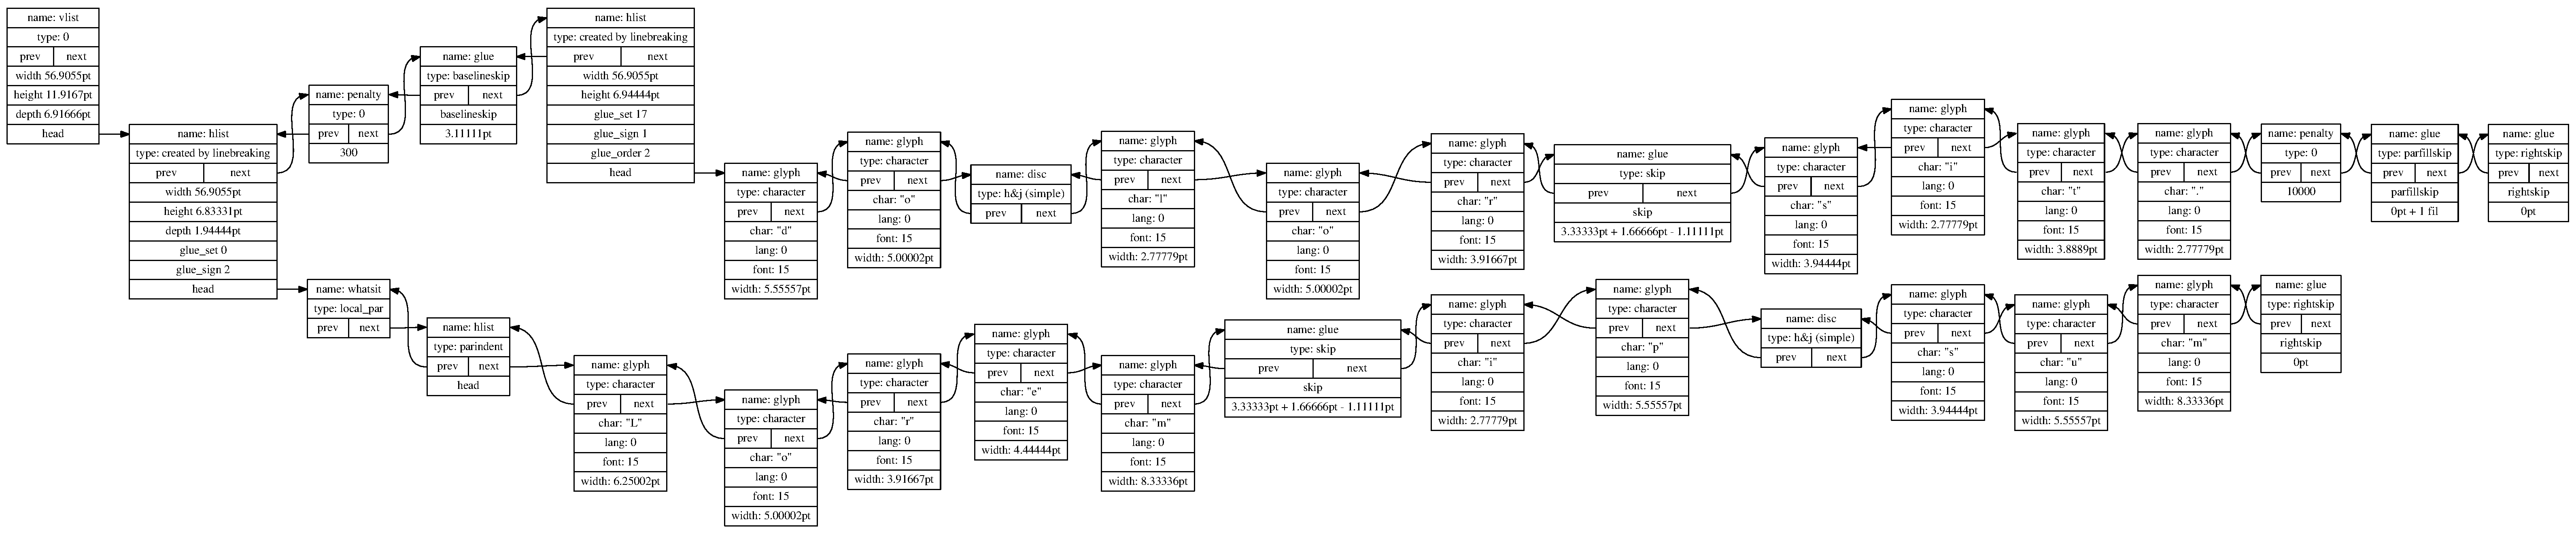
\includegraphics[width=\linewidth]{graphics/par}
%
% \paragraph{Tabular environment}
%
% \noindent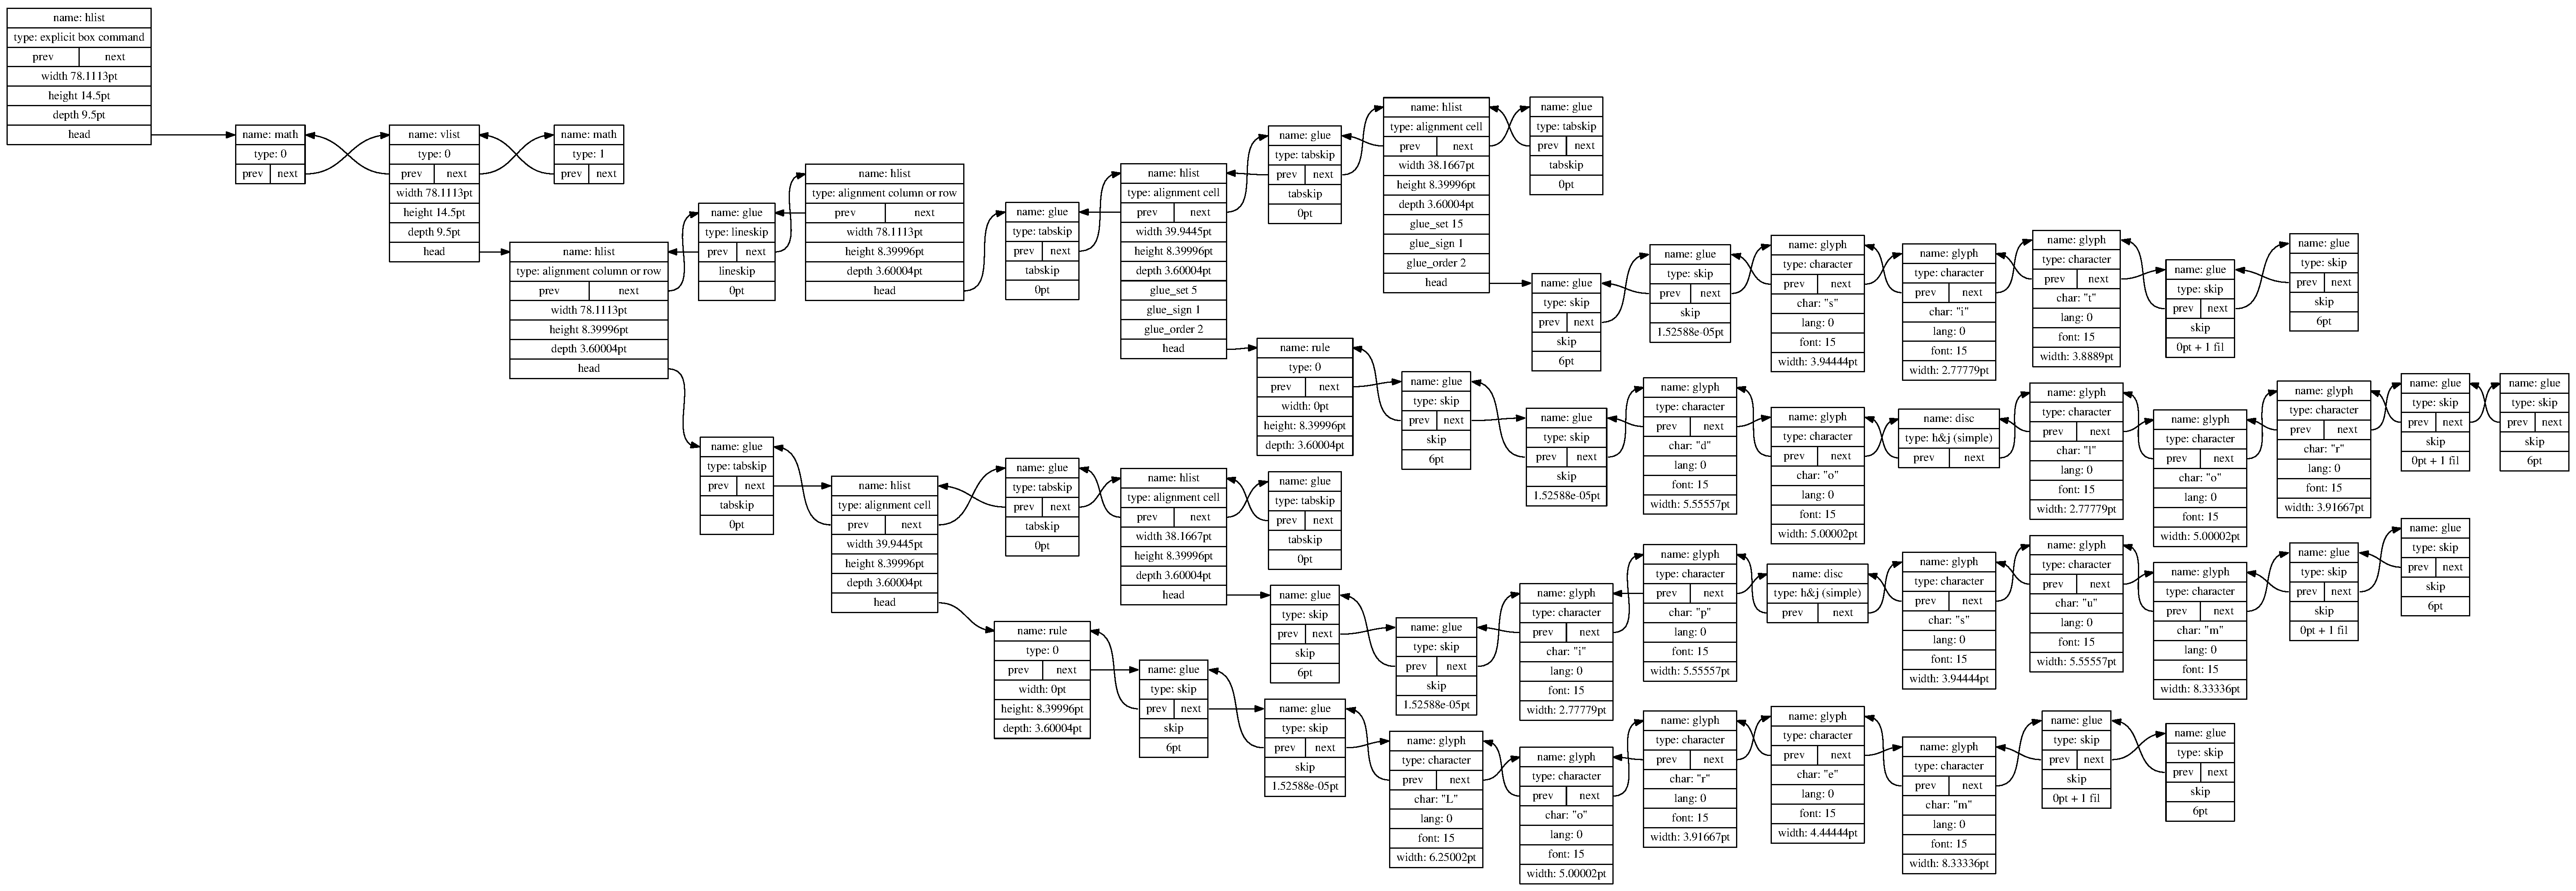
\includegraphics[width=\linewidth]{graphics/tabular}
%
% \paragraph{Picture environment}
%
% \noindent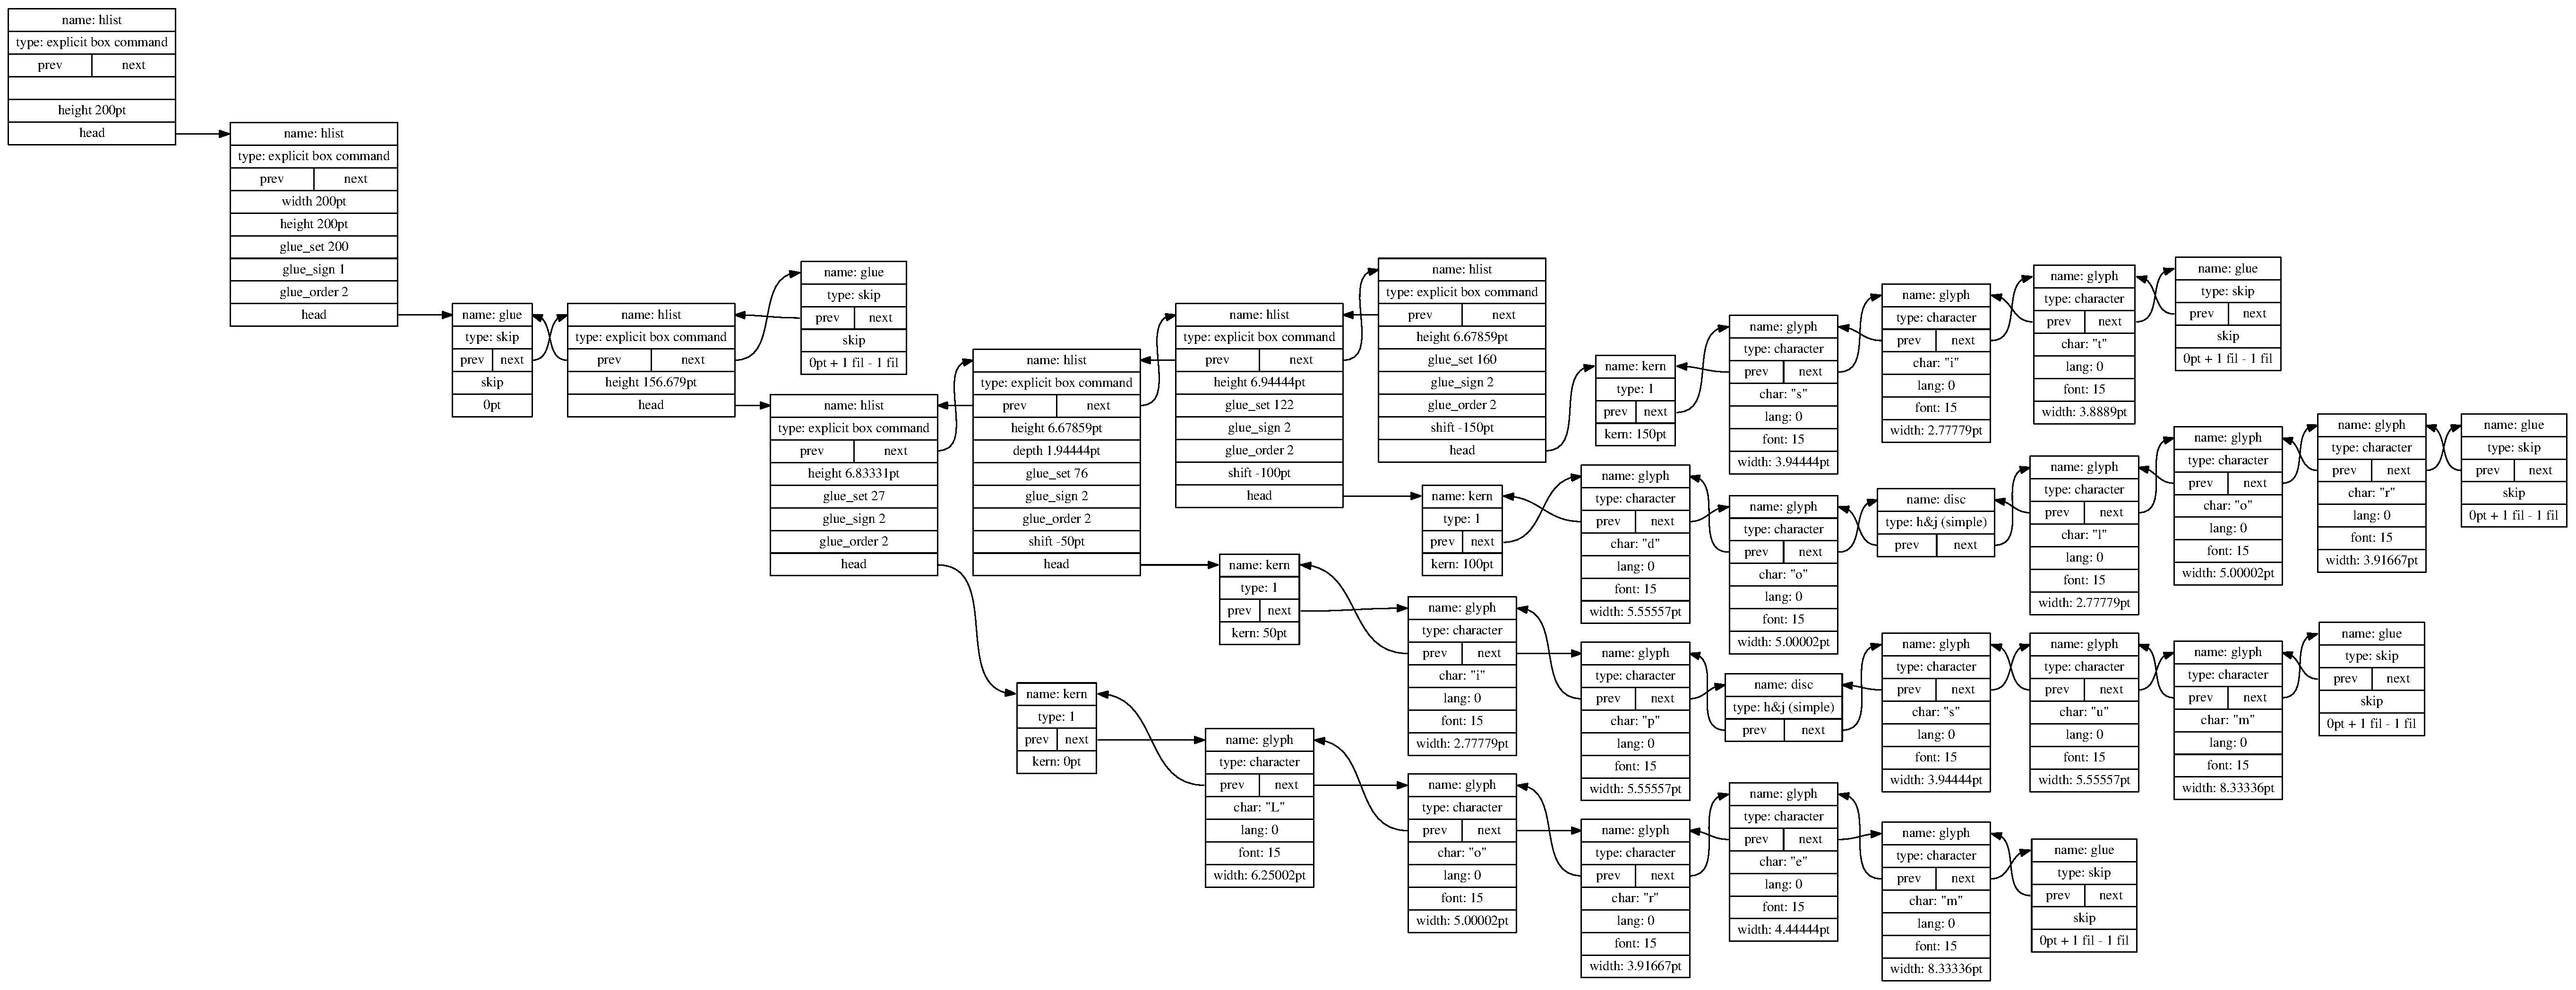
\includegraphics[width=\linewidth]{graphics/picture}
%
% \clozeluafunction{basic_make}
% The function |cloze.basic_make()| makes one gap. The argument |start|
% is the node, where the gap begins. The argument |stop| is the node,
% where the gap ends.
%    \begin{macrocode}
function cloze.basic_make(start, stop)
  local n = {}
  local l = {}
  n.head = start
  if not start or not stop then
    return
  end
  n.start = start
  n.stop = stop
  l.width = node.dimensions(
    cloze.status.hlist.glue_set,
    cloze.status.hlist.glue_sign,
    cloze.status.hlist.glue_order,
    n.start,
    n.stop
  )
  n.line = nodex.insert_line(n.start, l.width)
  n.color_text = nodex.insert_list('after', n.line, {nodex.create_color('text')})
  if registry.get_value_show() then
    nodex.insert_list('after', n.color_text, {nodex.create_kern(-l.width)})
    nodex.insert_list('before', n.stop, {nodex.create_color('reset')}, n.head)
  else
    n.line.next = n.stop.next
    n.stop.prev = n.line.prev
  end
%    \end{macrocode}
% I some edge cases the lua callbacks get fired up twice. After the
% cloze has been created, the start and stop whatsit markers can be
% deleted.
%    \begin{macrocode}
  registry.remove_marker(n.start)
  registry.remove_marker(n.stop)
end
%    \end{macrocode}
%
% \clozeluafunction{basic_search_stop}
% Search for a stop marker.
%    \begin{macrocode}
function cloze.basic_search_stop(head)
  local stop
  while head do
    cloze.status.continue = true
    stop = head
    if registry.check_marker(stop, 'basic', 'stop') then
      cloze.status.continue = false
      break
    end
    head = head.next
  end
  return stop
end
%    \end{macrocode}
%
% \clozeluafunction{basic_search_start}
% Search for a start marker. Also begin a new cloze, if the boolean
% value |cloze.status.continue| is true. The knowledge of the last
% hlist node is a requirement to begin a cloze.
%    \begin{macrocode}
function cloze.basic_search_start(head)
  local start
  local stop
  local n = {}
  if cloze.status.continue then
    n.hlist = nodex.search_hlist(head)
    if n.hlist then
      cloze.status.hlist = n.hlist
      start = cloze.status.hlist.head
    end
  elseif registry.check_marker(head, 'basic', 'start') then
    start = head
  end
  if start then
    stop = cloze.basic_search_stop(start)
    cloze.basic_make(start, stop)
  end
end
%    \end{macrocode}
%
% \clozeluafunction{basic_recursion}
% Parse recursivley the node tree. Start and stop markers can be nested
% deeply into the node tree.
%    \begin{macrocode}
function cloze.basic_recursion(head)
  while head do
    if head.head then
      cloze.status.hlist = head
      cloze.basic_recursion(head.head)
    else
      cloze.basic_search_start(head)
    end
      head = head.next
  end
end
%    \end{macrocode}
%
% \clozeluafunction{basic}
% The corresponding \LaTeX{} command to this lua function is \cmd{\cloze}
% \secref{sec:command-cloze}. The argument |head| is the head node of a
% node list.
%    \begin{macrocode}
function cloze.basic(head)
  cloze.status.continue = false
  cloze.basic_recursion(head)
  return head
end
%    \end{macrocode}
%
% \clozeluafunction{fix_length}
% Calculate the length of the whitespace before (|l.kern_start|) and
% after (|l.kern_stopt|) the text.
%    \begin{macrocode}
function cloze.fix_length(start, stop)
  local l = {}
  l.width = tex.sp(registry.get_value('width'))
  l.text_width = node.dimensions(start, stop)
  l.align = registry.get_value('align')
  if l.align == 'right' then
    l.kern_start = - l.text_width
    l.kern_stop = 0
  elseif l.align == 'center' then
    l.half = (l.width - l.text_width) / 2
    l.kern_start = - l.half - l.text_width
    l.kern_stop = l.half
  else
    l.kern_start = - l.width
    l.kern_stop = l.width - l.text_width
  end
  return l.width, l.kern_start, l.kern_stop
end
%    \end{macrocode}
%
% \clozeluafunction{fix_make}
% The function |cloze.fix_make| generates a gap of fixed width.
%
% \subparagraph*{Node lists}
%
% \subparagraph*{Show text:}
%
% \begin{nodelist}
% |n.start| & |whatsit| & |user_definded| & |index| \\
% |n.line| & |rule| &  & |l.width| \\
% |n.kern_start| & |kern| & & Depends on |align| \\
% |n.color_text| & |whatsit| & |pdf_colorstack| & Text color \\
%  & |glyphs| & & Text to show \\
% |n.color_reset| & |whatsit| & |pdf_colorstack| & Reset color \\
% |n.kern_stop| & |kern| & & Depends on |align| \\
% |n.stop| & |whatsit| & |user_definded| & |index| \\
% \end{nodelist}
%
% \subparagraph*{Hide text:}
%
% \begin{nodelist}
% |n.start| & |whatsit| & |user_definded| & |index| \\
% |n.line| & |rule| &  & |l.width| \\
% |n.stop| & |whatsit| & |user_definded| & |index| \\
% \end{nodelist}
%
% The argument |start| is the node, where the gap begins. The argument
% |stop| is the node, where the gap ends.
%    \begin{macrocode}
function cloze.fix_make(start, stop)
  local l = {} -- length
  local n = {} -- node
  l.width, l.kern_start, l.kern_stop = cloze.fix_length(start, stop)
  n.line = nodex.insert_line(start, l.width)
  if registry.get_value_show() then
    nodex.insert_list(
      'after',
      n.line,
      {
        nodex.create_kern(l.kern_start),
        nodex.create_color('text')
      }
    )
    nodex.insert_list(
      'before',
      stop,
      {
        nodex.create_color('reset'),
        nodex.create_kern(l.kern_stop)
      },
      start
    )
  else
    n.line.next = stop.next
  end
  registry.remove_marker(start)
  registry.remove_marker(stop)
end
%    \end{macrocode}
%
% \clozeluafunction{fix_recursion}
% Function to recurse the node list and search after marker. |head| is
% the head node of a node list.
%    \begin{macrocode}
function cloze.fix_recursion(head)
  local n = {} -- node
  n.start, n.stop = false
  while head do
    if head.head then
      cloze.fix_recursion(head.head)
    else
      if not n.start then
        n.start = registry.get_marker(head, 'fix', 'start')
      end
      if not n.stop then
        n.stop = registry.get_marker(head, 'fix', 'stop')
      end
      if n.start and n.stop then
        cloze.fix_make(n.start, n.stop)
        n.start, n.stop = false
      end
    end
    head = head.next
  end
end
%    \end{macrocode}
%
% \clozeluafunction{fix}
% The corresponding \LaTeX{} command to this Lua function is
% \cmd{\clozefix} \secref{sec:command-clozefix}. The argument |head| is
% the head node of a node list.
%    \begin{macrocode}
function cloze.fix(head)
  cloze.fix_recursion(head)
  return head
end
%    \end{macrocode}
%
% \clozeluafunction{par}
% The corresponding \LaTeX{} environment to this lua function is
% |clozepar| \secref{sec:command-clozepar}.
%
% \subparagraph*{Node lists}
%
% \subparagraph*{Show text:}
%
% \begin{nodelist}
% |n.strut| & |kern| &  & width = 0  \\
% |n.line| & |rule| &  & |l.width| (Width from hlist) \\
% |n.kern| & |kern| & & |-l.width| \\
% |n.color_text| & |whatsit| & |pdf_colorstack| & Text color \\
%  & |glyphs| & & Text to show \\
% |n.tail| & |glyph| &  & Last glyph in hlist \\
% |n.color_reset| & |whatsit| & |pdf_colorstack| & Reset color \\
% \end{nodelist}
%
% \subparagraph*{Hide text:}
%
% \begin{nodelist}
% |n.strut| & |kern| &  & width = 0 \\
% |n.line| & |rule| &  & |l.width| (Width from hlist) \\
% \end{nodelist}
%
% The argument |head| is the head node of a node list.
%    \begin{macrocode}
function cloze.par(head)
  local l = {} -- length
  local n = {} -- node
  for hlist in node.traverse_id(node.id('hlist'), head) do
    for whatsit in node.traverse_id(node.id('whatsit'), hlist.head) do
      registry.get_marker(whatsit, 'par', 'start')
    end
    l.width = hlist.width
    hlist, n.strut, n.head = nodex.strut_to_hlist(hlist)
    n.line = nodex.insert_line(n.strut, l.width)
    if registry.get_value_show() then
      nodex.insert_list(
        'after',
        n.line,
        {
          nodex.create_kern(-l.width),
          nodex.create_color('text')
        }
      )
      nodex.insert_list(
        'after',
        node.tail(head),
        {nodex.create_color('reset')}
      )
    else
      n.line.next = nil
    end
  end
  return head
end
%    \end{macrocode}
%
% \subsubsection{Basic module functions (base)}
%
% The |base| table contains functions which are published to the
% |cloze.sty| file.
%
% \clozeluafunction{register}
% This function registers the functions |cloze.par|, |cloze.basic| and
% |cloze.fix| the Lua callbacks. |cloze.par| and |cloze.basic| are
% registered to the callback |post_linebreak_filter| and |cloze.fix| to
% the callback |pre_linebreak_filter|. The argument |mode| accepts the
% string values |basic|, |fix| and |par|.
%    \begin{macrocode}
function base.register(mode)
  local basic
  if mode == 'par' then
    luatexbase.add_to_callback(
      'post_linebreak_filter',
      cloze.par,
      mode
    )
    return true
  end
  if not base.is_registered[mode] then
    if mode == 'basic' then
      luatexbase.add_to_callback(
        'post_linebreak_filter',
        cloze.basic,
        mode
      )
    elseif mode == 'fix' then
      luatexbase.add_to_callback(
        'pre_linebreak_filter',
        cloze.fix,
        mode
      )
    else
      return false
    end
    base.is_registered[mode] = true
  end
end
%    \end{macrocode}
%
% \clozeluafunction{unregister}
% |base.unregister(mode)| deletes the registered functions from the Lua
% callbacks. The argument |mode| accepts the string values |basic|,
% |fix| and |par|.
%    \begin{macrocode}
function base.unregister(mode)
  if mode == 'basic' then
    luatexbase.remove_from_callback('post_linebreak_filter', mode)
  elseif mode == 'fix' then
    luatexbase.remove_from_callback('pre_linebreak_filter', mode)
  else
    luatexbase.remove_from_callback('post_linebreak_filter', mode)
  end
end
%    \end{macrocode}
%
% Publish some functions to the |cloze.sty| file.
%    \begin{macrocode}
base.linefil = nodex.write_linefil
base.line = nodex.write_line
base.margin = nodex.write_margin
base.set_option = registry.set_option
base.set_is_global = registry.set_is_global
base.unset_local_options = registry.unset_local_options
base.reset = registry.unset_global_options
base.get_defaults = registry.get_defaults
base.get_value = registry.get_value
base.marker = registry.write_marker
%    \end{macrocode}
%
%    \begin{macrocode}
return base
%    \end{macrocode}
% \iffalse
%</lua>
% \fi
%
% \Finale
\endinput
